\documentclass{ifd-miniposter}
\usepackage{amsmath}
\usepackage{multicol}
\usepackage{multirow}
\usepackage{graphicx}
\usepackage{float}
\usepackage{comment}
\usepackage{listings}
\usepackage{xcolor} 
\usepackage{colortbl}
\usepackage{subcaption}

\usepackage{microtype}

\usepackage[T1]{fontenc} % Ensure proper encoding
\usepackage[utf8]{inputenc} % Ensure proper input encoding

%Setting up bibliography with natbib
\usepackage[numbers, authoryear]{natbib} % Use natbib for author-year citations
\bibliographystyle{plainnat} % Choose the bibliography style (authoryear)

% Hyperlinks settings
\usepackage[colorlinks=true, allcolors=blue]{hyperref}


% Settings
\lstset{ 
  language=Python, % specify the language
  frame=single, % adds a frame around the code
  backgroundcolor=\color{lightgray!20}, % set background color
  keywordstyle=\color{green}, % keyword style
  commentstyle=\color{blue}, % comment style
  stringstyle=\color{red}, % string literal style
  numbers=left, % where to put the line-numbers
  numberstyle=\tiny\color{gray}, % the style that is used for the line-numbers
  basicstyle=\ttfamily\footnotesize, % the size of the fonts that are used for the code
  breaklines=true, % automatic line breaking
  showstringspaces=false % do not show spaces in strings
}

% Title parameters
% title parameters
\thesisTitle{Discovering the Hardening Response of Lithium-Ion Pouch Cells Using Deep Learning}

\thesisStudent{Cédric Grieder}
\thesisType{Bachelor Thesis}
\thesisSupervisor{Dr. Xueyang Li, Dr. Thomas Tancogne-Dejean}

% Document
\begin{document}
% Title

\maketitle
\newpage
\thispagestyle{empty}
\null
\newpage
\section*{Abstract}
This thesis explores the application of deep learning, specifically fully connected neural networks (FCNN), to predict the hardening behavior of lithium-ion pouch cells under mechanical loading. Traditional two-stage analytical models often struggle to capture complex deformation responses, particularly in varied indentation scenarios. By integrating a neural network-based hardening law into finite element simulations, this study aims to improve the prediction of yield stress from plastic strain and enhance force-displacement matching.

This thesis introduces various feature selection methods, focusing on the gradient of the loss function. Various model configurations, machine learning hyperparameters, and selection methods are evaluated to optimize performance. The results demonstrate that while deep learning can effectively model and calibrate for a von Mises yield surface and its associated hardening response, there remains significant room for improvement in achieving consistent accuracy and stability.


\newpage
\tableofcontents
\newpage
\section{Introduction}
The increasing reliance on lithium-ion batteries, particularly in the automotive industry, necessitates the insurance of safety and performance of these energy storage systems. Lithium-ion pouch cells, widely used in electric vehicles, present specific challenges when subjected to mechanical loading. Large deformations of the mechanically loaded cells lead to potential safety hazards such as fire risks. Thus, modeling the mechanical behavior of these cells under mechanical load is crucial to predicting their response and mitigating potential risks.

Previous studies have used isotropic pressure-dependent plasticity models to describe the mechanical behavior of lithium-ion cells. However, these models often rely on simplified hardening laws that may not fully capture the complexity of the cell’s response to deformation. The hardening models, typically expressed through two-stage analytical models, may limit the ability to generalize the response under different loading conditions, particularly for complex geometries or diverse indentation scenarios. This thesis aims to overcome these limitations by leveraging deep learning techniques to predict the hardening response of lithium-ion pouch cells more accurately.

The primary objective of this research is to develop a neural network-based hardening law that can be integrated into finite element simulations, enabling more precise prediction of yield stress from plastic strain. By utilizing a fully connected neural network (FCNN), contrary to traditional hardening models and this approach relies on the neural network's ability to learn nonlinear relationships from data. The proposed model is designed to enhance computational efficiency while providing a more accurate representation of the material behavior, especially in complex indentation scenarios.

This thesis outlines the development of using a deep learning framework for calibrating the hardening law based on experimental data from indentation tests. The neural network is trained to predict the deformation resistance as a function of the equivalent plastic strain, with the calibration process relying on a fast simulation framework. The approach is further extended to investigate the performance of the model for various loading conditions and geometries.

In addition to the primary objective of improving force-displacement matching, this work explores the limitations of current modeling approaches, including convergence issues and the oscillating loss curves observed in previous studies. By incorporating machine learning into the calibration process, this research aims to establish a more robust and general framework for simulating the mechanical behavior of lithium-ion pouch cells. Thus, contributing to advancements in material science and battery technology \citep{Tancogne-Ind}.

\section{Methods}
The following section outlines the experimental and computational methods employed to investigate the mechanical behavior of lithium-ion pouch cells.

\subsection{Experiment}
This subsection describes the experimental setup, including the materials, indenter configurations, and procedures used to gather data for training the neural network model.
\subsubsection{Performed Experiments}
A series of indentation experiments are performed on 4Ah lithium-ion pouch cells, as described in \citet{Tancogne-Ind}. This is further illustrated by the balance of forces sketch in Figure \ref{fig:experimental_setup}.

\begin{figure}[ht]
    \centering
    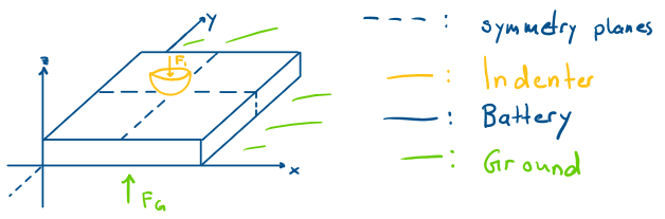
\includegraphics[width=0.5\linewidth]{graphics/sketch_experiment_setup.png}
    \caption{Experiment sketch}
    \label{fig:experimental_setup}
\end{figure}

The pouch cells used in the experiments are dimensions of 65.2 mm $\times$ 58.6 mm $\times$ 5.07 mm. The experiments include hemispherical indentations with indenter tip radii of 2.5 mm, 5 mm, 10 mm, 15 mm, 25 mm, and 50 mm, and cylindrical indentations with rod diameters of 5 mm, 10 mm, and 15 mm.
To facilitate clear identification of the various experiments, we introduce the following nomenclature: H\_D stands for hemispherical indentation, and C\_D denotes cylindrical indentation with indenter diameter $D$ mm respectively. For example, C\_10 refers to a cylindrical indentation using an indenter with a 10 mm diameter. The tests are conducted under quasi-static conditions, which imply no time-dependent kinematic effects.

\subsubsection{Data Preparation}
The experimental data is processed to focus on the relevant phase of the indentation. Specifically, the data is clipped to start from the initial contact between the indentation tool and the battery cell, defined by the condition where the indenter displacement is equal to zero. Subsequently, the data is truncated at the point of maximum force ($F_{\text{max}}$), where the applied force ($F_{\text{exp}}$) reaches it's peak. After partitioning, the time index is normalized so that the data begins at $t_0 = 0$, ensuring consistency across all experiments.


\subsection{Experiment Simulation}
%H_10_Simulation
\begin{figure}[ht]
    \centering
    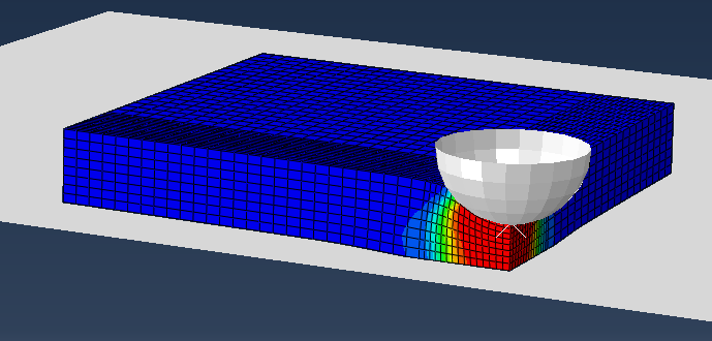
\includegraphics[width=0.5\linewidth]{graphics/Simulation_H10_overview.png}
    \caption{H\_10 Simulation}
    \label{fig:H_10_Simulation}
\end{figure}
Figure \ref{fig:H_10_Simulation} showcases the simulation setup of an H\_10 experiment.

Abaqus/Explicit is used to model the battery indentation experiment. To reduce computational time a special mesh is configured. Finite elements, which are presumed to be highly affected by the indenter, have a smaller element size than the rest of the model. Henceforth, this element set will be referred to as \enquote{output elements}. Output elements are a size of 0.4mm in both x and y direction and 8 elements in the battery z dimension. The other elements are a size 1.2mm in x, 1mm in y direction and 8 elements for the thickness in z direction.

%output_elements_nodes
\begin{figure}[ht]
    \centering
    \newlength{\textwidthSBStwo}
    \setlength{\textwidthSBStwo}{0.45\textwidth}
    
    \begin{minipage}[b]{\textwidthSBStwo}
        \centering
        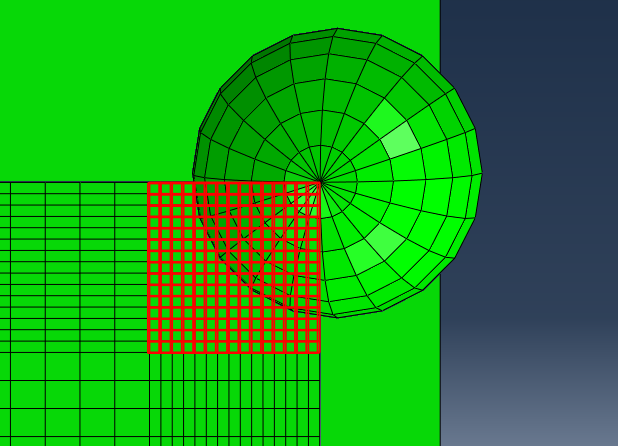
\includegraphics[width=\textwidthSBStwo]{graphics/output_extraction.PNG}
    \end{minipage}
    \hfill
    \begin{minipage}[b]{\textwidthSBStwo}
        \centering
        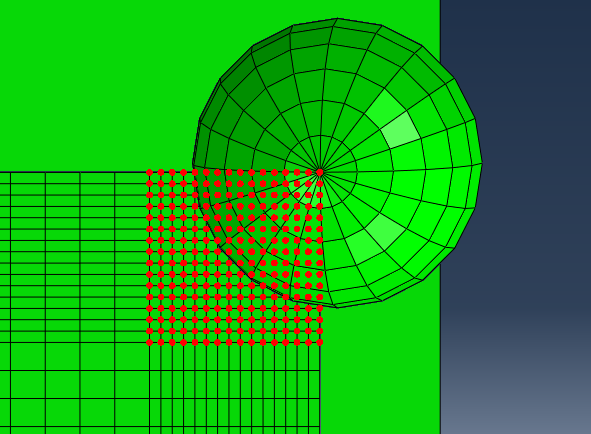
\includegraphics[width=\textwidthSBStwo]{graphics/output_extraction_nodes.PNG}
    \end{minipage}
    
    \caption{Output element (l) and node set (r)}
    \label{fig:output_elements_nodes}
\end{figure}

History output is requested for the output elements and corresponding node set, as illustrated in Figure \ref{fig:output_elements_nodes}. Extracted variables of the output elements are the stress tensor ($\sigma$), plastic strain ($\epsilon_p$), von Mises stress ($\sigma_{\text{vm}}$). Furthermore, the displacement vector of the output nodes $u_{\text{nodes}}$, z-displacement $u_3$ and z-reaction-force $F_{\text{R3}}$ of the indenter.
Default field output is requested for the whole model. 

The experiments are conducted under quasi-static conditions therefore mass scaling may be increased, as long as the kinetic energy compared to the total energy has a minor influence (<5\%). Mass scaling is applied with a minimal time increment of $d_t := 0.05s$.

The indenter is placed with a 0.1mm spacing to the battery top surface, in the midpoint of the battery's top $xy$-surface. The midpoint is chosen as \citet{Tancogne-Ind} showed that the geometrical placement of the indenter has a negligible influence on the force response. 

%Indentation_depths_of_experiments
\begin{table}[ht]
    \centering
    \begin{tabular}{c|c}
        \textbf{Experiment type} &  \textbf{Indentation depth [mm]}\\ \hline
         H\_10 &  1.88 \\ \hline
         H\_50 &  2.01      \\ \hline
         C\_20 &  1.10    \\  \hline
    \end{tabular}
    \caption{Indentation depths of simulated experiments}
    \label{tab:Indentation_depths_of_experiments}
\end{table}

To further reduce computational time, the symmetry of the battery is exploited and only a quarter of the battery is modeled. Symmetry boundary conditions are applied at the symmetry cut surfaces. The indenter tool and experiment table are modeled as analytical rigid surfaces. Furthermore, the table is fixed in all directions, whereas the indenter is constrained to move in negative z direction only by the specified amplitude. The smooth step amplitude is chosen with varying amplitude maxima depending on the experimental displacement of the respective indentation tool. Table \ref{tab:Indentation_depths_of_experiments} shows the effective indentation displacements (deducted of initial spacing) for performed simulations.

\begin{table}[ht]
\centering
\begin{tabular}{|c|c|}
\hline
$\epsilon_p$ & $\sigma_y$ [MPa] \\
\hline
0.0 & 100 \\
0.1 & 120 \\
0.2 & 200 \\
0.3 & 250 \\
0.4 & 270 \\
0.5 & 290 \\
0.6 & 300 \\
\hline
\end{tabular}
\caption{Copper hardening table}
\label{tab:copper_table}
\end{table}


The battery is modeled as a homogeneous solid, using global friction coefficient as proposed by \citet{Tancogne-Ind}. For the elastic definition of the homogenous battery material Young's modulus $E = 4200 \, \text{MPa}$ and Poisson's ratio $v = 0.1$ is chosen as previously indicated by \citet{Chung2018}. For the initial setup of the simulation a simple copper hardening table, shown in Table \ref{tab:copper_table} is used to define plasticity. This table will be overwritten by the neural network hardening law before every training process. The density ($\rho$) is assumed to correspond to a homogeneous mixture consisting of equal volumetric proportions (50/50) of copper and aluminum, yielding $\rho = 5.83 \times 10^{-9} \, \text{kg/mm}^3$, has no influence on the results as the simulation is conducted under quasi-static conditions.


\subsection{Neural Networks}
As a machine learning library, PyTorch is used due to its various built-in functions and user-friendly interface. This makes it a suitable choice for developing and experimenting with deep learning models.

As required by the task, a deep learning framework is developed to predict the hardening law. We use fully connected neural networks (FNNs), also known as multilayer perceptrons (MLPs), as they are straightforward to implement while being capable of handling complex data inputs and modeling nonlinearities effectively.

The hardening law will be modeled by a neural network denoted as \( k\text{-Neural-Network} \) (\(kNN\)). The neural network predicts the yield stress (\(\sigma_y\)) for a given plastic strain (\(\epsilon_p\)). Both \(\epsilon_p\) and \(\sigma_y\) are positive scalar values, thus the mapping behavior of the neural network can be expressed as:
\begin{align*}
kNN(\epsilon_p) : \mathbb{R}^+ \rightarrow \mathbb{R}^+, \quad \epsilon_p \mapsto \sigma_y.
\end{align*}

Neural networks are typically trained using an optimization algorithm known as gradient descent, which minimizes a loss function that quantifies the difference between the predicted and actual values. The process of updating the model's parameters, including its weights and biases, is known as backpropagation. This technique involves propagating the error gradient backward through the network to optimize learning \citep{bishop2006pattern}.
Given a set of training data \(\{(\epsilon_p^{(i)}, \sigma_y^{(i)})\}_{i=1}^N\), where \(N\) is the number of training samples, the loss function (\(L(\theta)\)) is defined as the mean squared error (MSE) between the predicted yield stress \(\hat{\sigma}_y^{(i)}\) and the true yield stress \(\sigma_y^{(i)}\):
\begin{align*}
L(\theta) &= \frac{1}{N} \sum_{i=1}^N \left(\hat{\sigma}_y^{(i)} - \sigma_y^{(i)}\right)^2,
\end{align*}
where \(\theta\) represents the set of all parameters (weights and biases) in the network.

To minimize the loss, the parameters \(\theta\) are updated iteratively using the gradient descent algorithm. The update rule for the weights \(w_{jk}\) in the network is given by:
\begin{align*}
w_{ij} \leftarrow w_{ij} - \eta \frac{\partial L(\theta)}{\partial w_{ij}},
\end{align*}
where \(\eta\) is the learning rate, a hyperparameter that controls the step size of each update.

Similarly, the biases \(b_i\) are updated as:
\begin{align*}
b_i \leftarrow b_i - \eta \frac{\partial L(\theta)}{\partial b_i}.
\end{align*}

Backpropagation computes the gradients \(\frac{\partial L(\theta)}{\partial w_{ij}}\) and \(\frac{\partial L(\theta)}{\partial b_i}\) by applying the chain rule of calculus to propagate the error backward from the output layer to the input layer. This enables the network to adjust its parameters in a way that minimizes the loss function.

The optimization and prediction capabilities of the neural network are therefore highly dependent on the accuracy of the gradient estimates and the effectiveness of the gradient descent scheme. The training process is wrapped in a loop called epochs, where the entire training dataset is passed through the network multiple times, allowing the model to learn and refine its predictions \citep{bishop2006pattern}.



\subsubsection{Mathematical Definitions}

The \textbf{Adam} (Adaptive Moment Estimation) optimization algorithm is defined as follows:

\begin{align}
m_t &= \beta_1 m_{t-1} + (1 - \beta_1) g_t \\
v_t &= \beta_2 v_{t-1} + (1 - \beta_2) g_t^2 \\
\hat{m}_t &= \frac{m_t}{1 - \beta_1^t} \\
\hat{v}_t &= \frac{v_t}{1 - \beta_2^t} \\
\theta_{t+1} &= \theta_t - \frac{\alpha \hat{m}_t}{\sqrt{\hat{v}_t} + \epsilon}
,
\end{align}

Where \(g_t\) is the gradient at time step \(t\), \(m_t\) and \(v_t\) are the first and second moment estimates, \(\beta_1\) and \(\beta_2\) are the exponential decay rates for these estimates, \(\alpha\) is the learning rate, \(\epsilon\) is a small constant to prevent division by zero, and \(\theta\) represents the parameters being optimized \citep{kingma2014adam}.
\label{Def:Adam}

\textbf{RMSprop} (Root Mean Square Propagation) is defined as:

\begin{align*}
v_t &= \beta v_{t-1} + (1 - \beta) g_t^2 \\
\theta_{t+1} &= \theta_t - \frac{\alpha}{\sqrt{v_t} + \epsilon} g_t,
\end{align*}

where \(v_t\) is the moving average of the squared gradients, \(\beta\) is the decay rate, and the other symbols have the same meanings as for Adam
\citep{hinton_lecture6a}.
\label{Def:RMSprop}


The \textbf{tanh} activation function is defined as:

\begin{align*}
\text{tanh}(x) &= \frac{\sinh(x)}{\cosh(x)} = \frac{e^x - e^{-x}}{e^x + e^{-x}}.
\end{align*}

The tanh function maps real-valued numbers into the range \((-1, 1)\) and is commonly used due to its ability to handle negative inputs and outputs symmetrically \citep{pytorch_tanh}.
\label{Def:tanh}

The \textbf{softplus} activation function is defined as:

\begin{align*}
\text{softplus}(x) &= \ln(1 + e^x)
\end{align*}

The softplus function is a smooth approximation of the ReLU function, providing a non-linear activation that maps inputs to positive outputs \citep{pytorch_softplus}.

\textbf{Gradient clipping} is a technique used to prevent the issue of exploding gradients, which may occur during backpropagation in deep neural networks. When gradients become excessively large, they can cause instability or divergence by making the model's weights update erratically. By ensuring that the gradient norms do not exceed a specified threshold, gradient clipping stabilizes the training process and allows the model to converge more reliably.

This technique is implemented using functions such as \texttt{clip\_grad\_norm}, which rescales the gradients (\(\nabla L(\theta)\)) if their \(L_2\) norm exceeds a given value, $c$:

\begin{align*}
\text{if } \|\nabla L(\theta)\|_2 > c, & \quad \nabla L(\theta) \leftarrow \nabla L(\theta) \times \frac{c}{\|\nabla L(\theta)\|_2}
\end{align*}

This ensures that the gradient vector's magnitude remains within the defined limits, effectively preventing the model from making overly large updates to its parameters. The function \texttt{clip\_grad\_norm} thus helps maintain stability during training, particularly in deep or recurrent models, promoting more controlled and stable learning \citep{pytorch_clip_grad_norm, zhang2020gradient}.

\label{Def:Clip}




\subsubsection{Model Definition}
Here the \texttt{SimpleModel} is defined, which corresponds to Model 3 from the chapter \ref{chap:model_selection} Model Selection.
Further the \texttt{DeepModel} is defined here which is similar to \texttt{SimpleModel} incorporating two more hidden layers for increased model complexity.

\paragraph{SimpleModel}
The layers in this model are structured as follows:
\begin{itemize}
    \item \textbf{Input Layer:} The input layer (\texttt{fc1}) consists of a linear transformation from 1 to 8 neurons.
    \item \textbf{Hidden Layers:} The network contains two hidden layers:
    \begin{itemize}
        \item \texttt{fc2}: 8 neurons to 16 neurons.
        \item \texttt{fc3}: 16 neurons to 8 neurons.
    \end{itemize}
    \item \textbf{Output Layer:} The final layer (\texttt{fc4}) reduces the output to a single neuron, followed by a \texttt{Softplus} activation to ensure the output is positive.
\end{itemize}

\paragraph{DeepModel}
The \texttt{DeepModel} builds upon the \texttt{SimpleModel} by introducing additional layers, increasing the depth and capacity of the network. The architecture is as follows:
\begin{itemize}
    \item \textbf{Input Layer:} The input layer (\texttt{fc1}) has 8 neurons, the same as in \texttt{SimpleModel}.
    \item \textbf{Hidden Layers:} The network features four hidden layers:
    \begin{itemize}
        \item \texttt{fc2}: 8 neurons to 16 neurons.
        \item \texttt{fc3}: 16 neurons to 32 neurons.
        \item \texttt{fc4}: 32 neurons to 16 neurons.
        \item \texttt{fc5}: 16 neurons to 8 neurons.
    \end{itemize}
    \item \textbf{Output Layer:} The final layer (\texttt{fc6}) outputs a single neuron, followed by the \texttt{Softplus} activation function, similar to \texttt{SimpleModel}.
\end{itemize}
Like \texttt{SimpleModel}, \texttt{DeepModel} employs Xavier initialization with \texttt{Tanh} activation gain and zero biases. The deeper architecture is intended to capture more complex relationships within the data, making \texttt{DeepModel} suitable for tasks requiring higher model capacity.

In the chapter \ref{chap:model_selection} Model Selection, a description is given why this model structure was chosen. The \texttt{SimpleModel} is referenced as Model 3.





\subsection{Model Selection}

\subsubsection{Optimization on Two-Stage Hardening Law}

To ensure adequate complexity of the chosen machine learning model structure, in this first model selection phase the training capability of different model structures, activation functions and deepness of the model are tested.
To test the fitting capability the two-stage-hardenining law used previously by \citet{Tancogne-Ind} shall be learned by the model.
Expressing the Loss as the mean square error of $\sigma_y$ and $\sigma_{two-stage}$, the predicted yield stress and the two stage hardening law:

\begin{align*}
L(\theta) &= \frac{1}{n} \sum_{i=1}^{n} \left( \sigma_y^{(i)} - \sigma_{\text{two-stage}}^{(i)} \right)^2
.
\end{align*}

The two stage hardening law from \citep{Tancogne-Ind} is defined as:

\begin{align*}
\begin{aligned}
&k_{\text{two-stage}}(\epsilon_p) = k_0 + \Delta k \\
&\Delta k(\epsilon_p) =
\begin{cases}
\begin{aligned}
A(\epsilon_p)^n & \text{if } \epsilon_p \leq \epsilon_c \\
A\epsilon_c^n + B(\epsilon_p - \epsilon_c) + Q\left(1 - \exp\left(-\beta(\epsilon_p - \epsilon_c)\right)\right) & \text{if } \epsilon_p > \epsilon_c ,
\end{aligned}
\end{cases}
\end{aligned}
\end{align*}

with parameters
\begin{align*}
\beta &= \frac{An\epsilon_c^{n-1} - B}{Q} \\
k_0 &= 0.1 \, \text{MPa}, \quad A = 1436 \, \text{MPa}, \quad n = 1.606 \\
B &= 6.3 \, \text{MPa}, \quad Q = 1.0 \, \text{MPa}.
\end{align*}


\subsubsection{Selection Process}
\label{chap:model_selection}
\begin{figure}[ht]
    \centering
    \newlength{\textwidthSelection}
    \setlength{\textwidthSelection}{0.32\textwidth}
    
    \begin{minipage}{\textwidthSelection}
    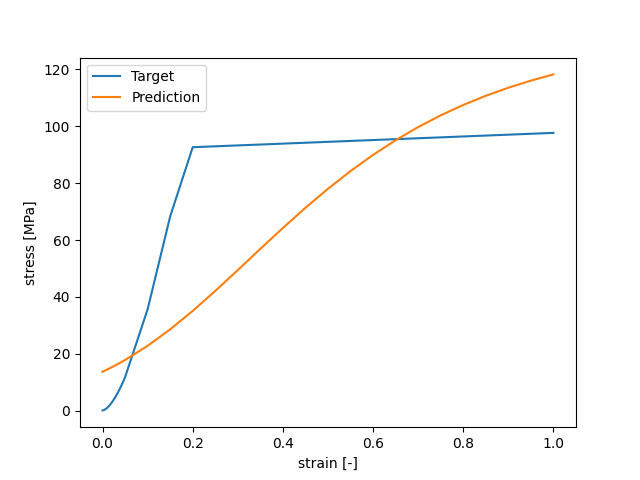
\includegraphics[width=\textwidth]{graphics/model1_target_prediction_comparison.png}
    \caption*{Model 1: 1-8-1 structure}
    \end{minipage}
    \hfill
    \begin{minipage}{\textwidthSelection}
    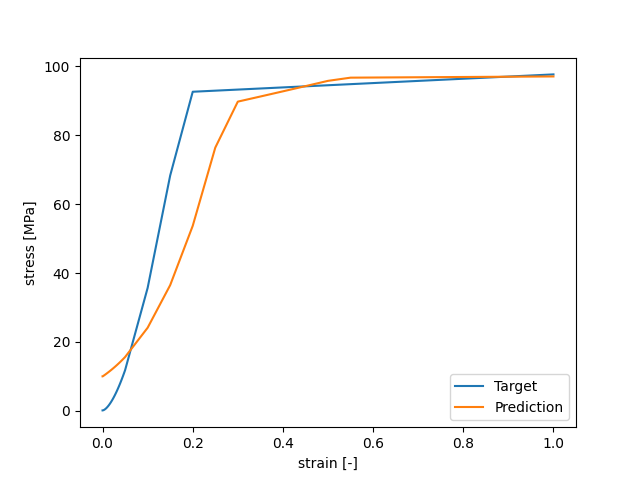
\includegraphics[width=\textwidth]{graphics/model2_hardening_target_vs_prediction.png}
    \caption*{Model 2: 1-8-16-1 structure}
    \end{minipage}
    \hfill
    \begin{minipage}{\textwidthSelection}
    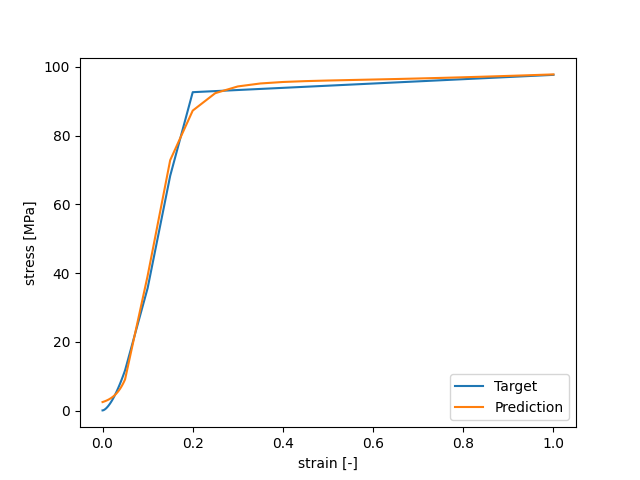
\includegraphics[width=\textwidth]{graphics/model_3_target_prediction_comparison.png}    
    \caption*{Model 3: 1-8-16-8-1 structure}
    \end{minipage}
    \hfill

    \caption{Performance of models with increasing complexity, Blue: Two-stage hardening law. Orange: model yield stress prediction}
    \label{fig:Selection_comparison}
\end{figure}


Sytematic exploration of various model configurations by incrementally increasing the number of layers and experimenting with different activation functions is performed.

The architectures tested consist of: Model 1 (\texttt{1-8-1-softplus}),
Model 2 (\texttt{1-8-16-1-softplus}), 
and Model 3 (\texttt{1-8-16-8-1-softplus}).
For each model, the performance using the activation functions \texttt{tanh}, \texttt{ReLU}, \texttt{Sigmoid}, and \texttt{GELU} is evaluated. Each configuration is trained over 1000 epochs utilizing a variety of optimization algorithms, including Adam, Adadelta, Adagrad, RMSprop, SGD, AdamW, and NAdam, with a consistent learning rate of 0.001.

After extensive experimentation, Model 3 with the \texttt{tanh} activation function, using Adam and RMSprop opimization algorithms, provided a "good fit" to the data, demonstrating superior performance across the tested configurations. To illustrate the progression of model complexity, the results of the 3 models with \texttt{tanh} using the RMSprop optimizer are showcased in Figure \ref{fig:Selection_comparison}.

A bottleneck structure refers to a architecture in neural networks where a layer (or a set of layers) has fewer neurons than the preceding and succeeding layers. This constrains the amount of information that can pass through, forcing the network to learn more efficient and abstract representations of the input data.

This selected model structure aligns with established findings on the role of information flow in feedforward neural networks, highlighting the abstraction capabilities of a fully connected neural network using a bottleneck structure \citep{Khadivi2016}.



\newpage
\subsection{Loss Function}
The overall goal is to closely aproximate the experimental force ($F_{\text{exp}}$) with the simulated force ($F_\text{{sim}}$), therefore a minimization of the difference between these quantities should be achieved.

The loss function is defined as the mean squared error of simulated force and the true experimental force over all indenter displacements ($U$).

\begin{align*}
L(\theta) &= \frac{1}{U} \sum_{u=0}^{u_{\text{max}}} \left(F_{\text{sim},u} - F_{\text{exp},u}\right)^2
.
\end{align*}

Recalling the definition of the hardening law: $kNN(\epsilon_p)\rightarrow \sigma_y$, it becomes evident that in order to perform backpropagation we need to relate $F_{\text{sim}}$ to $kNN$.

The weight update rule reads:

\begin{align*}
w_{ij} \leftarrow w_{ij} - \eta \frac{\partial L(\theta)}{\partial w_{ij}}
.
\end{align*}

Applying the chain rule yields following expression for the gradient of the loss with respect to the parameter weights:

\begin{align*}
    \frac{\partial L(\theta)}{\partial w_{ij}} = \frac{\partial L(\theta)}{\partial F_{\text{sim}}}\frac{\partial F_{\text{sim}}}{\partial w_{ij}}.
\end{align*}

Differentiating the loss with respect to $F_{\text{sim}}$ at a specific displacement:
\begin{align*}
    \frac{\partial L(\theta)}{\partial F_{\text{sim}}} = 2( F_{\text{sim}} - F_{\text{exp}}).
\end{align*}

The partial derivative \(\frac{\partial F_{\text{sim}}}{\partial w_{ij}}\) cannot be obtained analytically, as \(F_{\text{sim}}\) is a nonlinear function derived from the input of the hardening law using the Abaqus simulation. The gradient \(\frac{\partial F_{\text{sim}}}{\partial w_{ij}}\) is expressed in terms of \(\frac{\partial \sigma_y}{\partial w_{ij}}\), which represents the gradient of the model output and can be directly calculated using backpropagation.


\begin{figure}[ht]
    \centering
    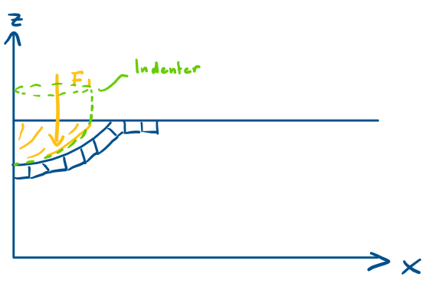
\includegraphics[width=0.5\linewidth]{graphics/2d_sketch_xz_plane.png}
    \caption{2D sketch xz-plane}
    \label{fig:2D_sketch_xz_plane}
\end{figure}

Figure \ref{fig:2D_sketch_xz_plane} shows a sketch of the surface distributed force (orange) of the indenter exerted on the battery model and deformed finite elements (blue) at a specific displacement.

The static balance of forces of the total indenter force and battery reaction force in z-direction reads:
\begin{align*}
    0 = F_{\text{indenter}} + F_{\text{battery}}\\
\end{align*}

The battery reaction force is the simulated force:
\begin{align*}
    F_{\text{battery}} &= F_{\text{sim}}\\
    F_{\text{sim}} &= -F_{\text{indenter}}.
\end{align*}

Writing the battery reaction force as a sum of $n$ elements forces leads to
\begin{align*}
    F_{\text{sim}} = \sum_{k=0}^{n_{\text{elements}}} F_{z\text{,element, } k}.
\end{align*}

%deformed_element_sketch
\begin{figure}[H]
    \centering
    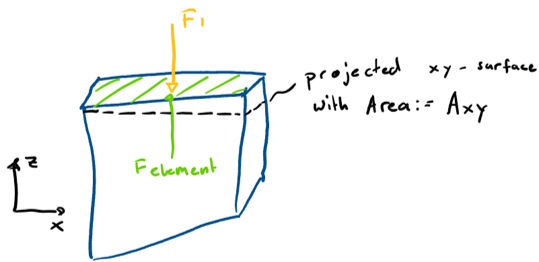
\includegraphics[width=0.5\linewidth]{graphics/deformed_element_sketch.png}
    \caption{Deformed element sketch}
    \label{fig:deformed_element_sketch}
\end{figure}

Figure \ref{fig:deformed_element_sketch} shows a sketch of a single deformed element with element force (green) and the projected xy-area of this element.

Expressing the element force in z direction as the product of stress in force direction and the normal area yields:
\begin{align*}
    F_{z, \text{element}} &= \sigma_{33} A_{xy}, \\
    F_{\text{sim}} &= \sum_{k=0}^{n_{\text{elements}}} (\sigma_{33} A_{xy})_k.
\end{align*}

Applying the chain rule for \(\frac{\partial F_{\text{sim}}}{\partial w_{ij}}\), assuming $A_{xy}$ to be constant results in
\begin{align*}
    \frac{\partial F_{\text{sim}}}{\partial w_{ij}} = 
    \sum_{k=0}^{n_{\text{elements}}}
    A_{xy, k}\frac{\partial \sigma_{33, k}}{\partial w_{ij}}.
\end{align*}

Applying the chain rule leads to an expression \(\frac{\partial F_{\text{sim}}}{\partial w_{ij}}\) in terms of \(\frac{\partial \sigma_y}{\partial w_{ij}}\):
\begin{align*}
    \frac{\partial F_{\text{sim}}}{\partial w_{ij}} = 
    \sum_{k=0}^{n_{\text{elements}}}
    A_{xy, k}
    \frac{\partial \sigma_{33, k}}{\partial \sigma_y}
    \frac{\partial \sigma_y}{\partial w_{ij}}.
\end{align*}

Writing the gradient for the weight update for a single element at a specific displacement enables us to rewrite as follows:
\begin{align*}
    \frac{\partial L(\theta)}{\partial w_{ij}} = 
    \frac{\partial L(\theta)}{\partial F_{\text{sim}}}
    A_{xy}
    \frac{\partial \sigma_{33}}{\partial \sigma_y}
    \frac{\partial \sigma_y}{\partial w_{ij}}
    .
\end{align*}

The gradient $\frac{\partial \sigma_{33}}{\partial \sigma_y}$ is dependent on the yield surface. Using the von Mises yield criterion, we write:
\begin{align*}
    \sigma_y &= \sigma_{\text{vM}}
    .
\end{align*}

The von Mises stress \(\sigma_{\text{vM}}\) is expressed as:

\[
\sigma_{\text{vM}} = \sqrt{\frac{1}{2} \left[ (\sigma_{11} - \sigma_{22})^2 + (\sigma_{22} - \sigma_{33})^2 + (\sigma_{33} - \sigma_{11})^2 \right] + 3\left(\sigma_{12}^2 + \sigma_{23}^2 + \sigma_{31}^2\right)}.
\]

To differentiate \(\sigma_{\text{vM}}\) with respect to \(\sigma_{33}\), the von Mises stress is first rewritten as a square root function:

\[
\sigma_{\text{vM}} = \sqrt{g(\sigma_{11}, \sigma_{22}, \sigma_{33}, \sigma_{12}, \sigma_{23}, \sigma_{31})},
\]

where

\[
g(\sigma_{11}, \sigma_{22}, \sigma_{33}, \sigma_{12}, \sigma_{23}, \sigma_{31}) = \frac{1}{2} \left[ (\sigma_{11} - \sigma_{22})^2 + (\sigma_{22} - \sigma_{33})^2 + (\sigma_{33} - \sigma_{11})^2 \right] + 3\left(\sigma_{12}^2 + \sigma_{23}^2 + \sigma_{31}^2\right).
\]

The chain rule is then applied to obtain the derivative:

\[
\frac{\partial \sigma_{\text{vM}}}{\partial \sigma_{33}} = \frac{1}{2\sigma_{\text{vM}}} \cdot \frac{\partial g}{\partial \sigma_{33}}.
\]

Next, the partial derivative of \(g\) with respect to \(\sigma_{33}\) is computed. The terms involving \(\sigma_{33}\) are:

\[
\frac{\partial g}{\partial \sigma_{33}} = \frac{1}{2} \cdot 2 \left[(\sigma_{33} - \sigma_{22}) + (\sigma_{33} - \sigma_{11})\right] = (\sigma_{33} - \sigma_{22}) + (\sigma_{33} - \sigma_{11}).
\]

Simplifying then yields:

\[
\frac{\partial g}{\partial \sigma_{33}} = 2\sigma_{33} - (\sigma_{11} + \sigma_{22}).
\]

Substituting this expression into the chain rule result gives:

\[
\frac{\partial \sigma_{\text{vM}}}{\partial \sigma_{33}} = \frac{2\sigma_{33} - (\sigma_{11} + \sigma_{22})}{\sigma_{\text{vM}}}.
\]

Inverting the derivative results in:

\[
\frac{\partial \sigma_{33}}{\partial \sigma_{\text{vM}}} = 
\frac{\sigma_{\text{vM}}}{2\sigma_{33} - (\sigma_{11} + \sigma_{22})}
=    \frac{\partial \sigma_{33}}{\partial \sigma_y}.
\]

This expression represents the inverse of the derivative of the von Mises stress with respect to the stress component \(\sigma_{33}\).

Finally an expression for the total gradient of the loss function with respect to the model weights is found:
\begin{align*}
    \frac{\partial L(\theta)}{\partial w_{ij}}=
    \sum_{u=0}^{u_{\text{max}}}
    \frac{\partial L(\theta)}{\partial F_{\text{sim}}}\Big|_u
    \sum_{k=0}^{n_{\text{elements}}}
    A_{xy}
    \frac{\partial \sigma_{33}}{\partial \sigma_y}
    \frac{\partial \sigma_y}{\partial w_{ij}}\Big|_k.
\end{align*}


\subsection{Filter Contact Elements}
The filter functions purpose is to select the finite elements that are in direct contact with the indenter tool to get an accurate description of the loss function gradient, ($\frac{\partial L(\theta)}{\partial w_{ij}}$).

As plastic strain $\epsilon_p$ is influenced by both geometry and material behavior, the plastic strain for a hardening law $kNN$ is considered dependent on indenter displacement ($u_3$) as well as the material properties. Elements that have an impact on the force response must undergo plastic strain. However, the condition $\epsilon_p > 0$ fails to filter the correct elements, as some elements deform due to stresses that are not aligned with the force direction.

Further elements which have a direct impact on the force response are expected to have a negative stress normal to the indenter force: $sign(\sigma_{33}) = - sign(F_\text{indenter}) = sign(F_\text{battery})$.

However the condition $\sigma_{33} < 0$ fails to filter the correct elements, as some elements experience a negative stress in force direction due to shear stresses of neighbouring elements.

Using the identified conditions, a filtering function may be found with a dynamic threshold for both plastic strain $\epsilon_p$ and stress in force direction $\sigma_{33}$.

The contact elements are distinguished according to the following criteria:

1. \textbf{Initial Condition and Contact-Based Inclusion}: 
   The set of contact elements \( C \) is initially empty at \( u_3 = 0 \). As the displacement \( u_3 \) increases, elements that are not filtered (according to the criteria described below) are added to this set. An element \( i \) is included in further analysis if it belongs to the set of contact elements \( C \). Mathematically, this is expressed as:
   \[
   i \in C,
   \]
   where \( C \subset E \), and \( E \) is the set of all elements.

2. \textbf{Strain-Based Filtering}:
   If an element \( i \) is not in contact with the indenter surface (i.e., \( i \notin C \)), it is filtered out if its strain \( \epsilon_i \) is below the current strain threshold \( \epsilon_{\text{threshold}} \). The strain threshold is defined dynamically based on the displacement \( u_3 \) as:
   \[
   \epsilon_{\text{threshold}}(u_3) = \epsilon_{\text{min}} + \frac{u_3}{u_{3,\text{max}}} \cdot (\epsilon_{\text{max}} - \epsilon_{\text{min}}).
   \]
   Hence, the strain-based filtering condition is:
   \[
   i \notin C \quad \text{and} \quad \epsilon_i < \epsilon_{\text{threshold}}(u_3).
   \]


\textbf{Combined Filtering Logic}

The overall filtering function is mathematically described by the set of filtered elements \( F \) as follows:

\[
F = \{ i \in E \mid (i \notin C) \wedge [(\epsilon_i < \epsilon_{\text{threshold}}(u_3)) \vee (\sigma_{33,i} > \sigma_{\text{threshold}}(u_3))] \}.
\]

This indicates that an element \( i \) is filtered out (i.e., added to the set \( F \)) if not in the contact set \( C \). Entailing that either its strain \( \epsilon_i \) is below the dynamic strain threshold or its stress component \( \sigma_{33,i} \) exceeds the dynamic stress threshold.


\paragraph{Updating Contact Elements}
Elements that are not filtered out are added to the contact set \( C \) as the displacement \( u_3 \) increases. Thus, the set \( C \) is updated dynamically throughout the simulation.

\paragraph{Elements Not Filtered Out}
The elements that remain for further analysis are those that satisfy the following condition:

\[
i \in C \quad \text{or} \quad \left[ i \notin F \text{ and } (\epsilon_i \geq \epsilon_{\text{threshold}}(u_3)) \text{ and } (\sigma_{33,i} \leq \sigma_{\text{threshold}}(u_3)) \right].
\]

\textbf{Threshold Definitions}

Minimum and maximum thresholds that yield promising results are:

\begin{itemize}
    \item \(\epsilon_{\text{min}} = 0.0008\) is the minimum strain threshold.
    \item \(\epsilon_{\text{max}} = 0.1\) is the maximum strain threshold.
    \item \(\sigma_{\text{min}} = -0.5 \text{ MPa}\) is the minimum stress threshold.
    \item \(\sigma_{\text{max}} = -5.0 \text{ MPa}\) is the maximum stress threshold.
\end{itemize}

The filter function using the specified threshold values is illustrated in Figure \ref{fig:Filter_function}.

%Filtering_mechanism_showcase

\begin{figure}[ht]
    \centering
    \newlength{\textwidthFilter}
    \setlength{\textwidthFilter}{0.192\textwidth}
    
    \begin{minipage}{\textwidthFilter}
    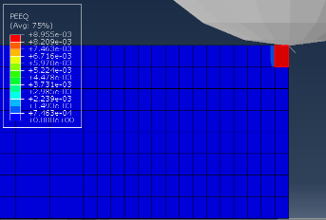
\includegraphics[width=\textwidth]{graphics/Filter_u0.png}    
    \end{minipage}
    \hfill
    \begin{minipage}{\textwidthFilter}
    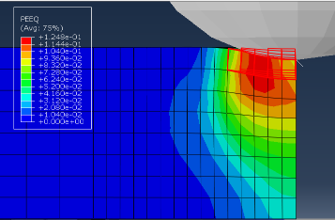
\includegraphics[width=\textwidth]{graphics/Filter_u1.png}    
    \end{minipage}
    \hfill
    \begin{minipage}{\textwidthFilter}
    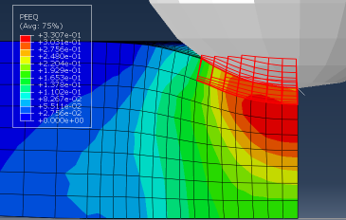
\includegraphics[width=\textwidth]{graphics/Filter_u2.png}    
    \end{minipage}
    \hfill
    \begin{minipage}{\textwidthFilter}
    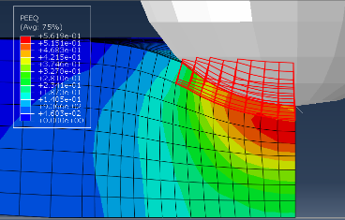
\includegraphics[width=\textwidth]{graphics/Filter_u3.png}    
    \end{minipage}
    \hfill
    \begin{minipage}{\textwidthFilter}
    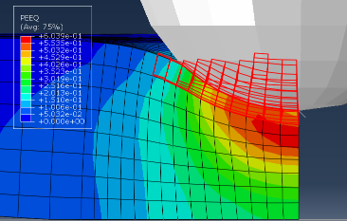
\includegraphics[width=\textwidth]{graphics/Filter_u4.png}    
    \end{minipage}
    \hfill

    \caption{Filter function, contact elements highlighted in red}
    \label{fig:Filter_function}
\end{figure}



\subsection{Neural Network Training}
This section details the training process for the neural network, including the experimental setup, data preprocessing, model initialization, and optimization techniques applied to predict the hardening behavior of lithium-ion pouch cells.

\subsubsection{Experiment}
The neural network is trained on the H\_10 experiment simulation. Opting for a hemispherical indenter with a radius of 5 mm offers a balance between resolution and computational complexity. A smaller indenter would require finer meshing, increasing computational costs, while a larger indenter might reduce the precision of local deformation details. Additionally, this indenter size has been experimentally validated by \citet{Tancogne-Ind}, providing the data for calibrating the hardening law. This moderate indenter size also ensures that the neural network generalizes effectively across different material behaviors.


\subsubsection{Scaling}

Input and output scaling is a critical step in neural network training as it ensures optimal model performance during the learning process. By scaling the input and output data to a consistent range, typically between 0 and 1, the network's weights are updated more evenly during backpropagation, reducing the likelihood of gradients vanishing or exploding. This can lead to faster convergence and improved model performance \citep[p.~8]{bishop2006pattern}. Scaling the data also helps the neural network to generalize better by preventing the model from becoming biased towards features with larger ranges.

In this particular case, the input scaling is determined by observing the maximum strain value in the Abaqus simulations, which is found to be approximately 0.55. To allow for some margin of error, the maximum value for scaling was set to 0.7. This ensures that even if the maximal strain increases slightly in future simulations, the model will still be able to handle the data without any issues. Similarly, the output scaling is determined by running a simulation based on the two-stage hardening model from \citep{Tancogne-Ind}. The maximum observed stress is around 100, so a maximum value of 120 is chosen for scaling, again allowing for some error margin. This careful consideration of the data ranges ensures that the model is robust and accurately predicts outputs even if the input or output values exceed those observed in the initial data set.


\subsubsection{Model Initialization}
In \citet{glorot2010} the Xavier (Glorot) initialization technique was introduced. Used to address the challenges of training deep neural networks, particularly the issues related to the vanishing and exploding gradients. Traditional random initialization methods often lead to poor convergence due to extreme variations in the layer activations and gradients, causing the network to either learn very slowly or get stuck in suboptimal solutions. The Xavier initialization method aims to maintain the variance of the activations and gradients across layers, ensuring that information flows properly through the network during training. This is achieved by initializing the weights with values drawn from a uniform distribution bounded by \(\pm \sqrt{\frac{6}{n_{\text{in}} + n_{\text{out}}}}\), where \(n_{\text{in}}\) and \(n_{\text{out}}\) are the number of input and output units in the layer, respectively. This careful initialization leads to faster convergence and better performance in deep networks.



\subsubsection{Model Prediction}

As Abaqus requires a table of strain-yield stress values to define the battery material hardening behavior, we use the kNN model to predict the yield stress for a predefined strain tensor. The chosen strain tensor \(\boldsymbol{\epsilon}_p\) is constructed to cover a wide continuous range of strain values. The strain tensor is defined as follows:

\begin{itemize}
    \item \textbf{Very small strains}: \( \epsilon_p \in [0, 0.00095] \) with a uniform spacing of \( \Delta \epsilon_p = 0.00005 \).
    \item \textbf{Small strains}: \( \epsilon_p \in [0.001, 0.0095] \) with a uniform spacing of \( \Delta \epsilon_p = 0.0005 \).
    \item \textbf{Medium strains}: \( \epsilon_p \in [0.01, 0.4] \) with a uniform spacing of \( \Delta \epsilon_p = 0.005 \).
    \item \textbf{Large strains}: \( \epsilon_p \in [0.42, 0.7] \) with a uniform spacing of \( \Delta \epsilon_p = 0.02 \).
\end{itemize}

These strain intervals are carefully chosen to ensure a smooth and continuous strain-yield stress relationship. The resulting strain tensor (\(\boldsymbol{\epsilon}_p\)) is formed by concatenating these intervals to provide a comprehensive set of strain values.

The kNN model, denoted as \( \text{kNN}(\boldsymbol{\epsilon}_p) \rightarrow \boldsymbol{\sigma}_y \), is then employed to predict the corresponding yield stress tensor (\(\boldsymbol{\sigma}_y\)). The yield stress tensor, is subsequently used to define the material's hardening behavior in Abaqus.

\subsubsection{Feature Selection}
Recalling the definition of the loss functions gradient:
\begin{align*}
    \frac{\partial L(\theta)}{\partial w_{ij}}=
    \sum_{u=0}^{u_{\text{max}}}
    \frac{\partial L(\theta)}{\partial F_{\text{sim}}}\Big|_u
    \sum_{k=0}^{n_{\text{elements}}}
    A_{xy}
    \frac{\partial \sigma_{33}}{\partial \sigma_y}
    \frac{\partial \sigma_y}{\partial w_{ij}}\Big|_k
    .
\end{align*}

The loss functions gradient for a single element at a specific indenter displacement ($u$) with plastic strain ($\hat{\epsilon_p}$):

\begin{align*}
    \frac{\partial L(\theta)}{\partial w_{ij}}\Big|_{\hat{\epsilon_p}} =
    \frac{\partial L(\theta)}{\partial F_{\text{sim}}}
    A_{xy}
    \frac{\partial \sigma_{33}}{\partial \sigma_y}
    \frac{\partial \sigma_y}{\partial w_{ij}}\Big|_{\hat{\epsilon_p}}
    .
\end{align*}

A single neural network input (\({\hat{\epsilon_p}}\)), combined with its corresponding gradient of the loss function \(\frac{\partial L(\theta)}{\partial w_{ij}}\Big|_{\hat{\epsilon_p}}\), will be referred to as a \textbf{feature}. This is analogous to classical machine learning, where a feature typically consists of an input (often denoted as \(x_i\)) and a target or true output (often denoted as \(y_i\)).


Recalling the gradient $\frac{\partial \sigma_{33}}{\partial \sigma_{\text{vM}}}$, which is a factor in the total loss function:

\begin{align*}
    \frac{\partial \sigma_{33}}{\partial \sigma_{\text{vM}}}=
    \frac{\sigma_{\text{vM}}}{2\sigma_{33} - (\sigma_{11} + \sigma_{22})}.
\end{align*}

For numerical stability $\tau << 1$ is added to the denumerator to avoid division by $0$:

\begin{align*}
    \frac{\partial \sigma_{33}}{\partial \sigma_{\text{vM}}}\approx
    \frac{\sigma_{\text{vM}}}{2\sigma_{33} - (\sigma_{11} + \sigma_{22})+\tau}.
\end{align*}

However for configurations where $(2\sigma_{33} - (\sigma_{11} + \sigma_{22})) \approx 0$ this gradient becomes very large and unstable.

Introducing the concept of \textbf{feature selectors}, where the gradient \(\frac{\partial \sigma_{33}}{\partial \sigma_{\text{vM}}}\) is adjusted, or features are added or removed to refine the model's performance.


\textbf{No selector}: Referencing "No Selector" means that the features are neither modified nor deleted.

\textbf{Regularization}: Regularization is a concept often used in machine learning where the loss function is modified to include additional terms that penalize certain model characteristics. The primary goal of regularization is to prevent overfitting by discouraging overly complex models that could perform well on training data but poorly on unseen data. This is typically achieved by adding a penalty term to the loss function, such as L1 (Lasso) or L2 (Ridge) regularization, which encourages sparsity in the model coefficients or reduces the magnitude of the coefficients, respectively. By controlling the complexity of the model, regularization helps improve generalization performance, leading to more robust predictions on new data \citep[pp.~256-259]{bishop2006pattern}.

\begin{figure}
    \centering
    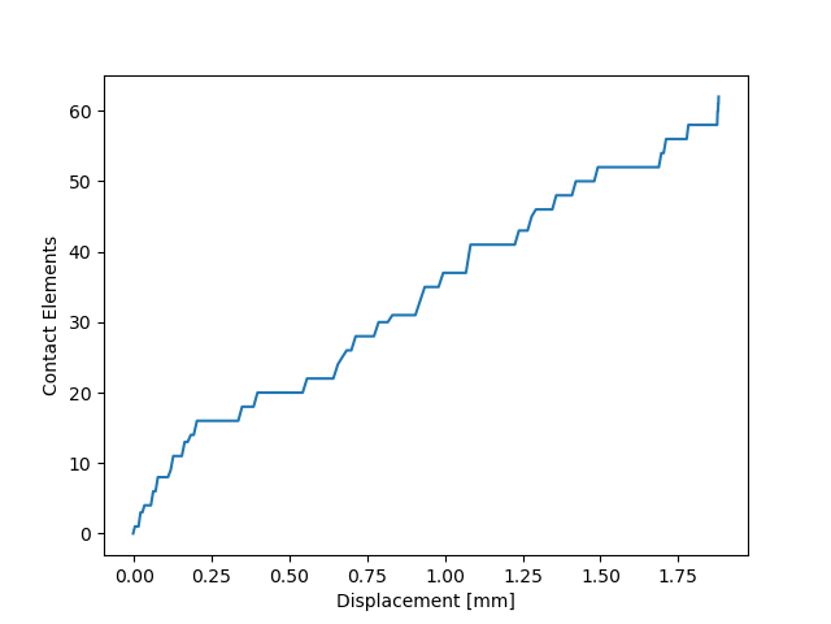
\includegraphics[width=0.5\linewidth]{graphics/contactelements_curve.png}
    \caption{Number of contact elements per displacement}
    \label{fig:n_elements_disp}
\end{figure}

To balance the number of input features per indenter displacement ($u$), particularly as with increasing displacements naturally due to the behaviour of the "contact elements filter", a method was implemented where \(\alpha\) additional features with ${\hat{\epsilon_p}} = 0$ as the input were introduced. This was motivated by the observation that the model did not adjust well to certain regions of the force-displacement curve, potentially due to the imbalance in features. See the number of input features per displacement in Figure \ref{fig:n_elements_disp}.

Denoting $n(u)$ the number of contact elements dependant on indenter displacement.The function of \(\alpha\) was calculated as:
\begin{align*}
    \alpha(u) = n(u_\text{max}) - n(u).
\end{align*}

Defining $k_0$ as $kNN(\hat{\epsilon_p}) = kNN(0)$ and further introducing a scaling factor $\lambda$ to tune the regularization effect. The gradient of the loss function for regularization features is written as:

\begin{align*}
    \frac{\partial L(\theta)}{\partial w_{ij}}\Big|_{\hat{\epsilon_p}}=
    \lambda k_0
    \frac{\partial L(\theta)}{\partial F_{\text{sim}}}
    \frac{\partial k_0}{\partial w_{ij}}.
\end{align*}

As a result the total loss function writes:

\begin{align*}
    \frac{\partial L(\theta)}{\partial w_{ij}}=
    \sum_{u=0}^{u_{\text{max}}}
    \frac{\partial L(\theta)}{\partial F_{\text{sim}}}\Big|_u
    \sum_{k=0}^{n_{\text{elements}}}
    A_{xy}
    \frac{\partial \sigma_{33}}{\partial \sigma_y}
    \frac{\partial \sigma_y}{\partial w_{ij}}\Big|_k 
    + 
    \alpha (u) \lambda k_0
    \sum_{u=0}^{u_{\text{max}}}
    \frac{\partial L(\theta)}{\partial F_{\text{sim}}}\Big|_u
    \frac{\partial k_0}{\partial w_{ij}}.
\end{align*}

Setting $\lambda = 0.1$ shows the best model performance in terms of loss compared to choosing $\lambda = 0.05$ and $\lambda = 1$.

This technique acts as a form of regularization, as it constrains the model by reducing the influence of features in regions with fewer active inputs, thereby promoting better generalization across the entire force-displacement curve.

\paragraph{Enforce Direction}
Another approach is to determine the expected direction of the gradient \(\frac{\partial \sigma_{33}}{\partial \sigma_{\text{vM}}}\) by reasoning through a simpler problem.


A simpler case is uniaxial compression, where load is uniformly applied to a sample and stresses act only in the principal direction, with the principal stress $\sigma_3$ aligned with the z-axis $\sigma_3 = \sigma_{33}$. For the unixial compression case follows:
\begin{align*}
    \sigma_{1} = \sigma_{11} = \sigma_{2} = \sigma_{22} = 0.
\end{align*}

For uniaxial compression we calculate the gradient with $\frac{\partial \sigma_{33}}{\partial \sigma_{\text{vM}}}$.

The von Mises stress for principal stresses is defined as:
\begin{align*}
    \sigma_\text{vM}=
    \sqrt{
    \frac{1}{2}
    [
    (\sigma_1 - \sigma_2)^2 + 
    (\sigma_2 - \sigma_3)^2 + 
    (\sigma_3 - \sigma_1)^2
    ]
    },   
\end{align*}

with $\sigma_{1} = \sigma_{2} = 0$ the expression further simplifies to:

\begin{align*}
    \sigma_\text{vM}=
    \sqrt{ \sigma_3^2
    }
    =
    |\sigma_3|.
\end{align*}

Since $\sigma_\text{vM}=|\sigma_3|$, $\frac{\partial \sigma_{3}}{\partial \sigma_{\text{vM}}}$ depends on the sign of $\sigma_3$:

\begin{itemize}
    \item if $ \sigma_3 > 0$:
    \begin{align*}
    \frac{\partial \sigma_{3}}{\partial \sigma_{\text{vM}}} =
    \frac{\partial \sigma_{3}}{\partial \sigma_3} = 1
    \end{align*}
    \item if $\sigma_3 < 0$:
    \begin{align*}
    \frac{\partial \sigma_{3}}{\partial \sigma_{\text{vM}}} =
    \frac{\partial \sigma_{3}}{\partial (-\sigma_3)} = -1
    \end{align*}.
\end{itemize}

Thus the gradient 
$\frac{\partial \sigma_{33}}{\partial \sigma_{\text{vM}}} = \frac{\partial \sigma_{3}}{\partial \sigma_{\text{vM}}}$ is expressed as:
\begin{align*}
\frac{\partial \sigma_{33}}{\partial \sigma_{\text{vM}}} =
\begin{cases}
1, & \text{if } \sigma_{33} > 0 \\
-1, & \text{if } \sigma_{33} < 0
\end{cases}
.
\end{align*}

From this we get the uniaxial compression relationship: $\frac{\partial \sigma_{33}}{\partial \sigma_{\text{vM}}}$ needs to have the same direction as $\sigma_{33}$ itself.

Let the set $S$ contain all features where $\operatorname{sign}(\frac{\partial \sigma_{33}}{\partial \sigma_{\text{vM}}}) \neq \operatorname{sign}(\sigma_{33}$) holds.

For the feature selector "Enforce Direction", features in $S$ are then modified as:
\begin{align*}
\frac{\partial \sigma_{33}}{\partial \sigma_{\text{vM}}}\Big|_S := \operatorname{sign}(\sigma_{33})
\end{align*}

\subsubsection{Backpropagation}

To practically perform backpropagation in PyTorch, features need to be represented as tensors. Opting to use one single tensor for the plastic strain input feature, further referenced as the strain tensor (\(\boldsymbol{\hat{\epsilon}_p}\)), and correspondingly one tensor for the gradient of the loss function feature, further referenced as the gradient tensor (\(\boldsymbol{\nabla L}\)). The model prediction, the yield stress tensor, is further referenced as the stress tensor. The stress tensor (\(\boldsymbol{\hat{\sigma}_y}\)) is mathematically given by \(kNN(\boldsymbol{\hat{\epsilon}_p}) \rightarrow \boldsymbol{\hat{\sigma}_y}\).


To illustrate how backpropagation is performed in PyTorch using a custom gradient tensor, a minimal code example is given, as this information was surprisingly hard to understand, but very easy to implement.\citep{pytorch_custom_gradient}

An example strain and gradient tensor are defined, the model is selected and an optimizer is chosen:
\begin{lstlisting}[language=Python]
#define the tensors
strain_tensor = torch.tensor([0.1, 0.12, 0.2])
grad_tensor = torch.tensor([-1, 0, 1])

#select the model
model = SimpleModel()
#choose the optimizer, set the learn rate to 0.001
optimizer = optim.Adam(model.parameters(), lr=0.001).
\end{lstlisting}

Further we let our model make a prediction on the strain tensor and capture the resulting stress tensor:

\mbox{$kNN(\boldsymbol{\hat{\epsilon}_p}) \rightarrow \boldsymbol{\hat{\sigma}_y}$},

\begin{lstlisting}[language=Python]
#perform prediction
stress_tensor = model(strain_tensor).    
\end{lstlisting}

Next, the gradient tensor is propagated backwards through the model on the predicted stress tensor, this is mathematically equivalent to calculating:
$
\frac{\partial L (\theta)}{\partial \boldsymbol{\hat{\sigma}_y}}
\frac{\partial \boldsymbol{\hat{\sigma}_y}}{\partial w_{ij}}
$,

\begin{lstlisting}
#backpropagation with custom gradient
stress_tensor.backward(grad_tensor)
\end{lstlisting}

Optionally, gradient clipping can be employed before updating the model weights:

\begin{lstlisting}
# apply gradient clipping
clip = 5
torch.nn.utils.clip_grad_norm(model.parameters(), clip)
\end{lstlisting}

Lastly, we update the model weights using the optimizer:
$w_{ij} \leftarrow w_{ij} - \mu \frac{\partial L (\theta)}{\partial w_{ij}}$,
\begin{lstlisting}
#updating the model weights
optimizer.step()
\end{lstlisting}


The features used in backpropagation to train the model are dependant on the \textit{feature selector} used. The mechanism however is the same for all features:
\begin{itemize}
    \item Choose an input feature dependant on indenter displacement $u$ and the element $\hat{\epsilon_p}(u, \text{element})$.
    
    \item Use the according \textit{feature selector} algorithm and calculate
    $\frac{\partial L (\theta)}{\partial \sigma_y}(\hat{\epsilon_p})$.
    
    \item Add the single features to the tensors: $\hat{\epsilon}_p \rightarrow \boldsymbol{\hat{\epsilon}_p}, \frac{\partial L (\theta)}{\partial \sigma_y}(\hat{\epsilon_p})
    \rightarrow \boldsymbol{\nabla L}$.

    \item Repeat until no features are left.

    \item Shuffle the tensors $\boldsymbol{\hat{\epsilon}_p}, \boldsymbol{\nabla L}$, which means randomizing their order to prevent possible issues due to a ordered dataset.

    \item Do a forward pass: $kNN(\boldsymbol{\hat{\epsilon}_p}) \rightarrow \boldsymbol{\hat{\sigma}_y}$.

    \item Perform backpropagation on the stress tensor with the gradient tensor: $\frac{\partial L (\theta)}{\partial \boldsymbol{\hat{\sigma}_y}}
\frac{\partial \boldsymbol{\hat{\sigma}_y}}{\partial w_{ij}}$.

    \item Apply gradient clipping if specified $\quad \nabla L(\theta) \leftarrow \nabla L(\theta) \times \frac{c}{\|\nabla L(\theta)\|_2}$ (\ref{Def:Clip}).

    \item Update the model weights using the optimizer:  $w_{ij} \leftarrow w_{ij} - \mu \frac{\partial L (\theta)}{\partial w_{ij}}$ (\ref{Def:Adam}).
    
\end{itemize}




\subsubsection{Training Loop}

%Training_loop
\begin{figure}[ht]
    \centering
    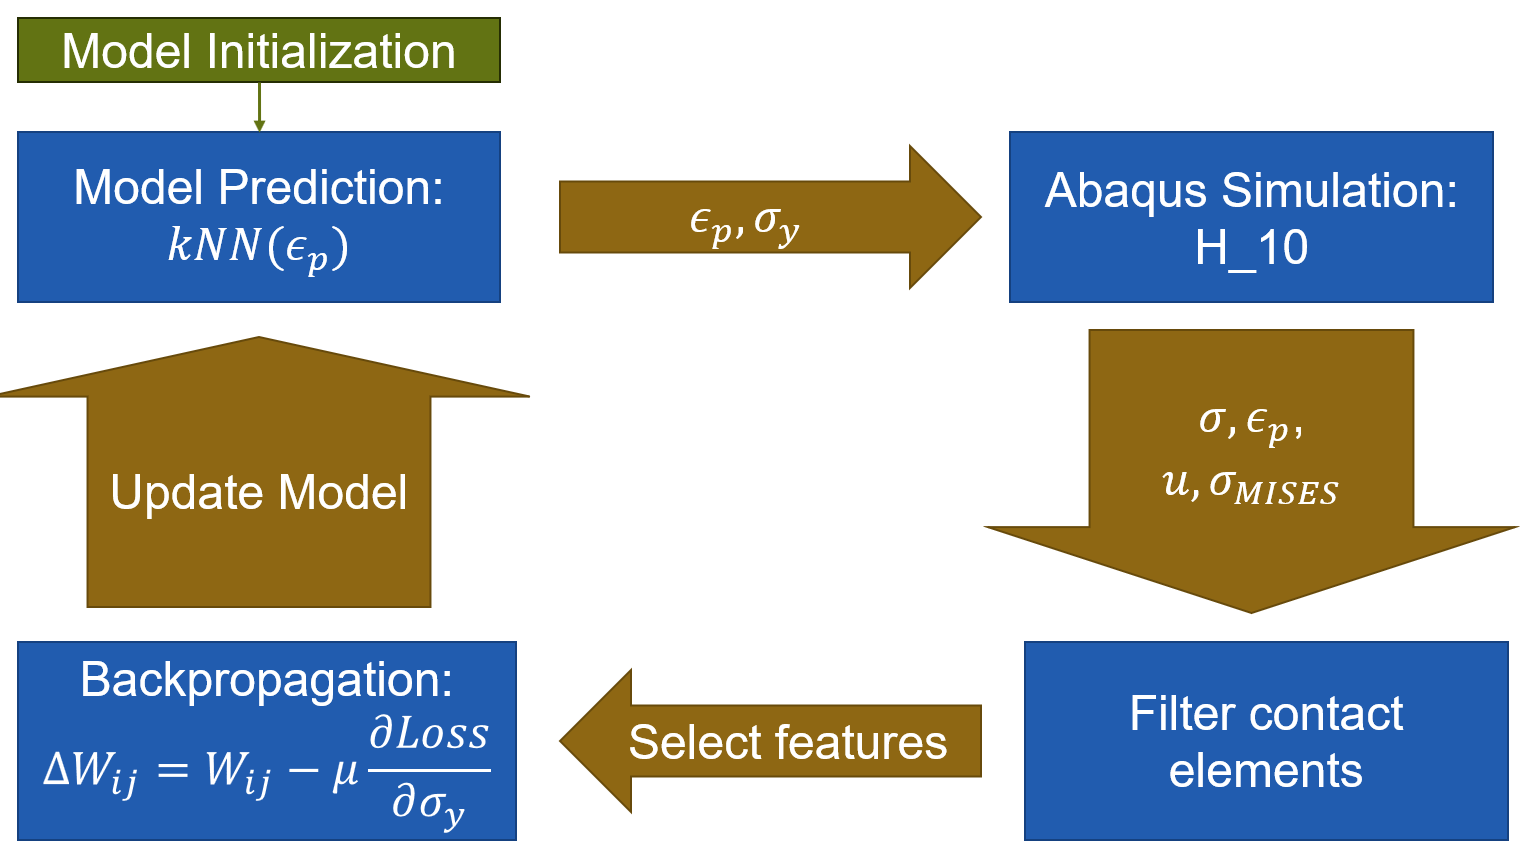
\includegraphics[width=0.5\linewidth]{graphics/Training_Loop_Schematic.PNG}
    \caption{Training loop}
    \label{fig:Training_loop}
\end{figure}

In the training loop, which is illustrated in Figure \ref{fig:Training_loop}, the chosen Neural Network model is trained on the features extracted from the Abaqus simulation. The training loop is run for a fixed number of epochs and a fixed configuration of the training parameters thereof being:

\begin{itemize}
    \item \textbf{Number of epochs}: How many times the training loop is run. When running training on 8 CPU's on the Euler HPC one epoch takes aproximately 1 minute. Depending on the \textit{feature selector}, clip value, learn rate, model, optimizer, the lowest loss / best hardening law ($kNN$) may be found earlier or later. Typically epoch number is kept between 100 and 1000, 1600 is the maximum value tested, showing no significant improvement compared to 1000.
    
    \item \textbf{Learn rate} ($lr$, $\mu$): different weight update parameter sizes were used, these are the initial learn rates which both RMSprop and Adam optimizer adjust based on the gradients, as described previously. Still the chosen value matters here, experimentation yielded $\mu \in \{10^{-3}, 5 \cdot 10^{-4}\}$ as the best performing values. Whilst higher values lead to unstable training behaviour and lower values give slow convergence for which the number of epochs becomes extensively high.

    \item \textbf{Clip value}: Tested values are: $\{\text{None}, 0.1, 0.5, 1, 2, 5, 10, 15\}$. Generally clip values lower than 5 yield similar results to very low learn rates, decreasing model convergence speed whilst not improving stability noticeably. Using no clip value generally makes the training process unstable and leads to divergent solutions. Clip values $\{5, 10, 15\}$ are primarily used as they balanced convergence and stability for the feature selectors: \textit{Regularization, Enforce Direction}
    
    Alternative clipping techniques are tested as well using \textit{No Selector} most notably:

    Directly clipping the gradient features (${\nabla L}$) if the absolute value exceeds a certain threshhold. No useful threshhold is found. Also scaling down loss gradients of features which has significant outlier values in its gradient ${\nabla L}$ (more than two standard deviations of all features in $\boldsymbol{\nabla L}$) does not improve the training behaviour.
\end{itemize}

\begin{figure}[ht]
    \centering
    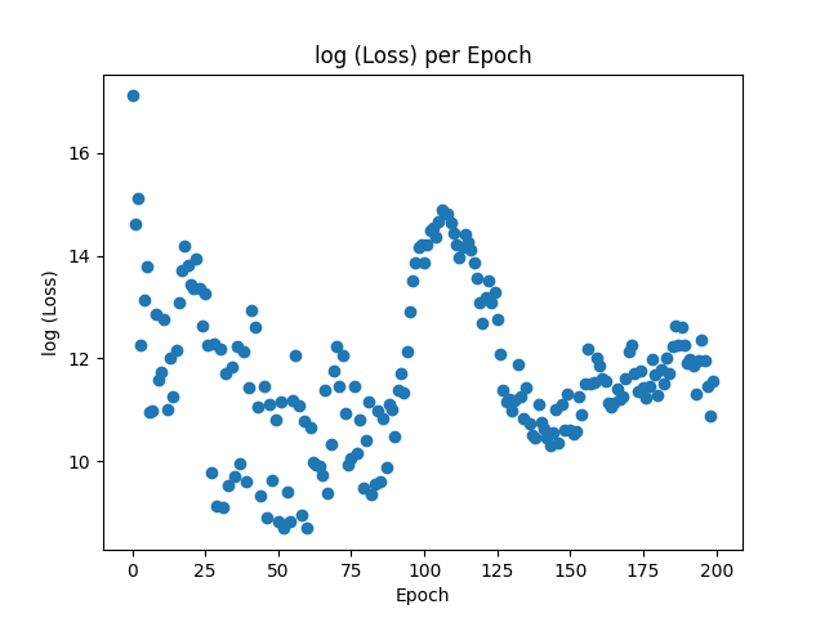
\includegraphics[width=0.5\linewidth]{graphics/log_loss_Deep_model_regularization.png}
    \caption{Logarithm of the loss against epoch number, \texttt{DeepModel}, \textit{Regularization}}
    \label{fig:logloss}
\end{figure}

As no specific training parameters are found which yield a monotonically decreasing loss curve and generally convergence is not achieved, meaning that the model starts diverging after reaching a local minima, the training loop is run for a fixed number of epochs. The best model is chosen after training, best meaning loss in terms of mean squared error of experimental and simulation force respectively. Figure \ref{fig:logloss} is showcasing an example loss curve, illustrating the non-monotonic behaviour.

\subsection{Validation}

\begin{figure}[h]
    \centering
    \newlength{\textwidthSBSthree}
    \setlength{\textwidthSBSthree}{0.3\textwidth}  % Reduce this from 0.25 to a lower value if necessary
    
    \begin{minipage}[b]{\textwidthSBSthree}
        \centering
        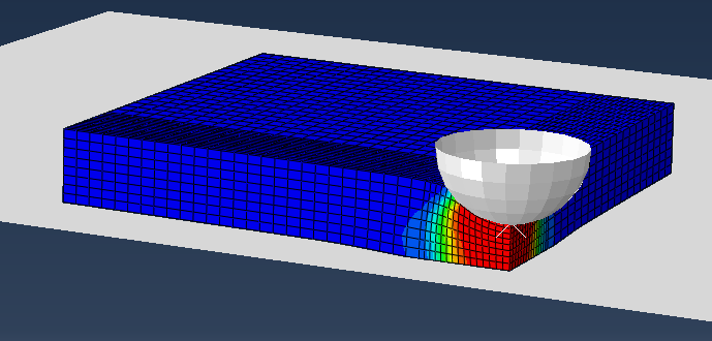
\includegraphics[width=\textwidthSBSthree]{graphics/Simulation_H10_overview.png}
    \end{minipage}
    \hfill
    \begin{minipage}[b]{\textwidthSBSthree}
        \centering
        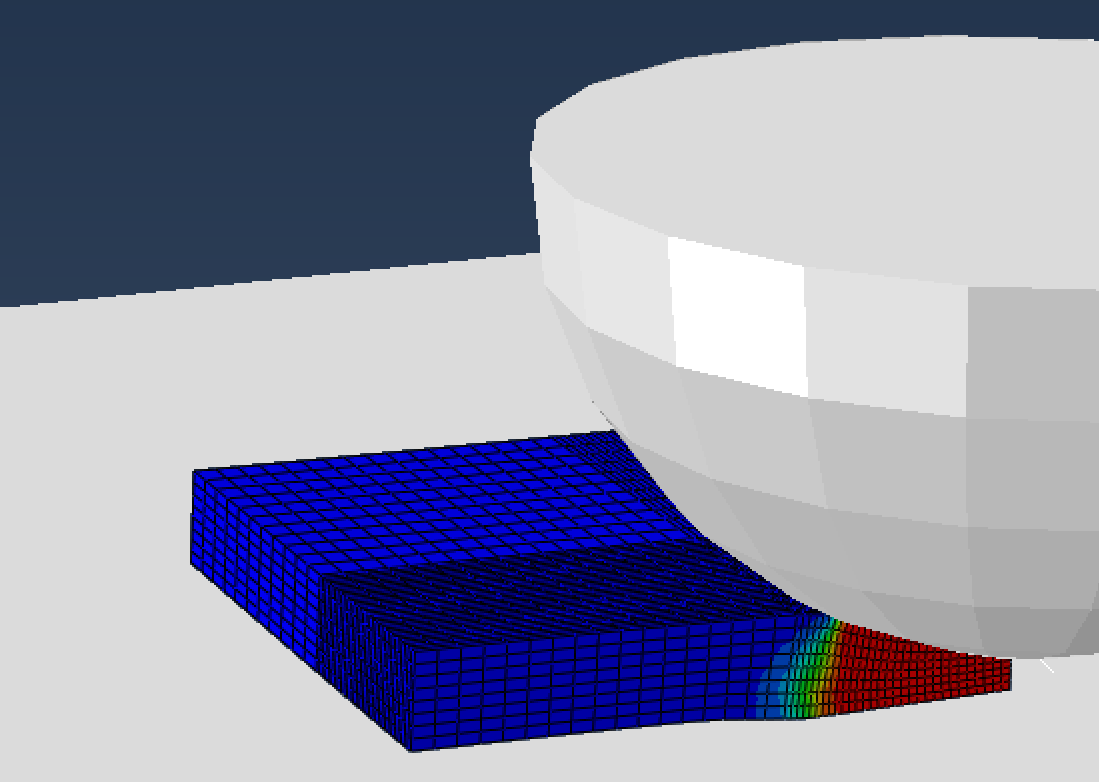
\includegraphics[width=\textwidthSBSthree]{graphics/H_50_overview.PNG}
    \end{minipage}
    \hfill
    \begin{minipage}[b]{\textwidthSBSthree}
        \centering
        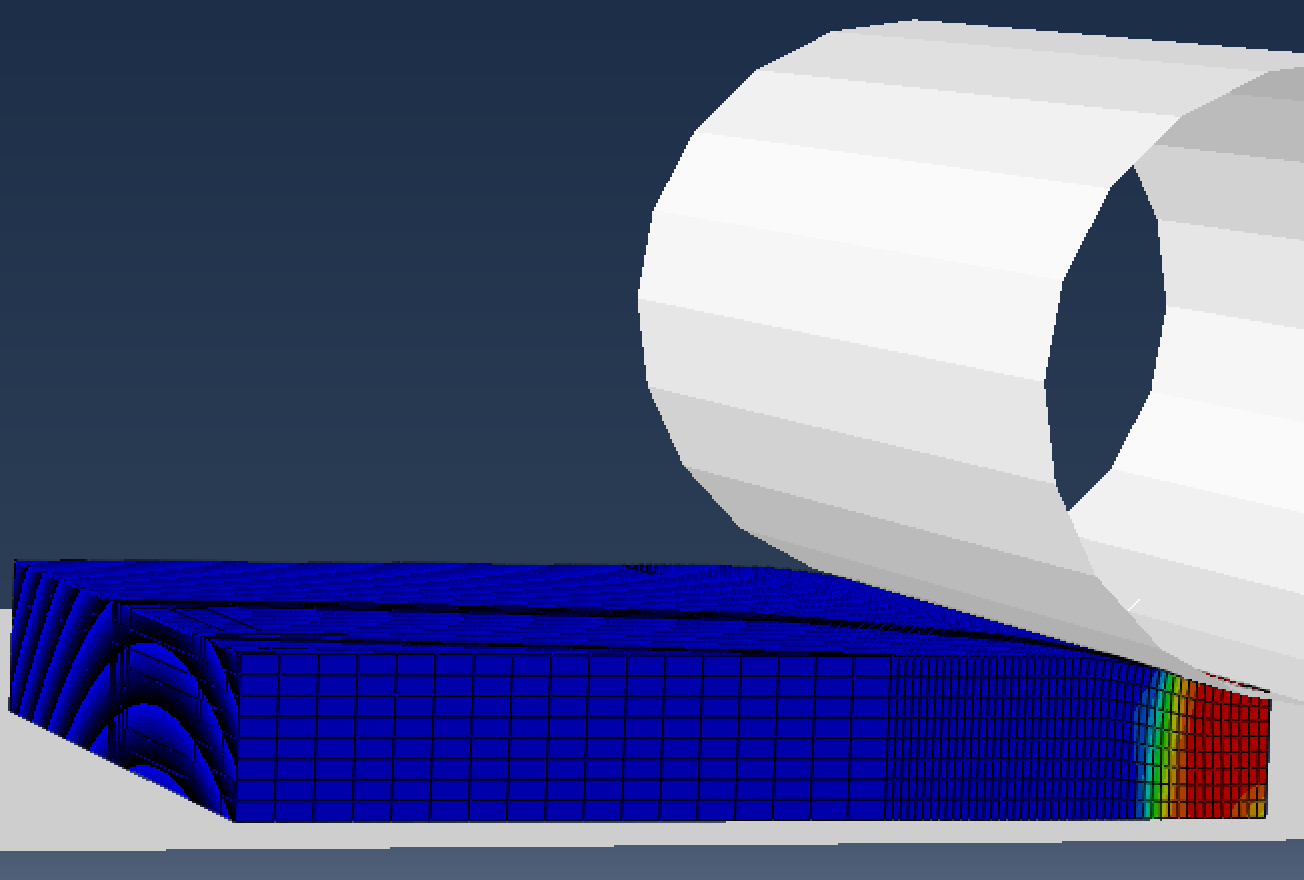
\includegraphics[width=\textwidthSBSthree]{graphics/C_20_overview.PNG}
    \end{minipage}
    \caption{H\_10, H\_50, C\_20 simulation setup (l) to (r)}
    \label{fig:various_experiments}
\end{figure}



For the validation of selected neural network hardening laws ($kNN$), validation runs are performed on H\_50 and C\_20 indentation experiment simulations. These are chosen as H\_50 reflects a significant size difference of the indenter tool and C\_20 reflects another shape and size (cylindrical instead of hemispherical). The three different simulation setups are illustrated in Figure \ref{fig:various_experiments}.

  
\section{Results}
\newlength{\textwidthMultiplier}
\setlength{\textwidthMultiplier}{0.45\textwidth}

This section presents the results obtained from evaluating the performance of the SimpleModel and DeepModel under various configurations, focusing on feature selection strategies, learning rates, optimizers, and gradient clipping techniques. The key performance metrics, including MAE, MAPE, and MSE, are used to assess and compare the models' effectiveness in minimizing the force error between the simulated and experimental results.

\subsection{Conducted Tests}

This section presents the performance evaluation of SimpleModel and DeepModel across the three previously introduced feature selection strategies. Each configuration is run for 600 epochs to ensure comparability. The learning rate is set at either 0.0005 or 0.001, with RMSprop used for the \textit{Regularization} configuration and Adam for the \textit{No Selector} and \textit{Enforce Direction} configurations. Gradient clipping values of 5, 10, and 15 are used for Regularization, No Selector, and Enforce Direction, respectively. These configurations are selected based on previous experiments to optimize the models' performance and to facilitate a balanced comparison.

\begin{table}[h]
    \centering
    \begin{tabular}{|c|c|c|c|c|c|}
        \hline
        \textbf{Model} & \textbf{Feature Selector} & \textbf{Learn rate (lr/{$\boldsymbol\mu$)}} & \textbf{Optimizer} & \textbf{Clipping Value} & \textbf{Epochs} \\ \hline
        SimpleModel & No Selector        & 0.001              & Adam      & 10             & 600    \\ \hline
        SimpleModel & Regularization     & 0.0005 / 0.001     & RMSprop   & 5              & 600    \\ \hline
        SimpleModel & Enforce Direction  & 0.001              & Adam      & 15             & 600    \\ \hline
        DeepModel   & No Selector        & 0.001              & Adam      & 10             & 600    \\ \hline
        DeepModel   & Regularization     & 0.0005 / 0.001     & RMSprop   & 5              & 600    \\ \hline
        DeepModel   & Enforce Direction  & 0.001              & Adam      & 15             & 600    \\ \hline
    \end{tabular}
    \caption{Comparison of SimpleModel and DeepModel across different feature selectors, learning rates, optimizers, and gradient clipping values.}
    \label{tab:configurations}
\end{table}



\subsection{Key Performance Metrics}
For the performance evaluation following metrics are used: The mean absolute error (MAE), the mean percentage error (MAPE) and the mean square error (MSE).Key performance metrics (KPM):
Lower Scalar results for all performance metrics mean "better results" in Terms of minimizing the force error between simulated and experimental force.

\begin{align*}
\text{MAE}(F_{\text{exp}}, F_{\text{sim}}) := \frac{1}{n} \sum_{i=1}^{n} |F_{\text{exp},i} - F_{\text{sim},i}|
\\
\text{MAPE}(F_{\text{exp}}, F_{\text{sim}}) := \frac{100\%}{n} \sum_{i=1}^{n} \left| \frac{F_{\text{exp},i} - F_{\text{sim},i}}{F_{\text{exp},i}} \right|
\\
\text{MSE}(F_{\text{exp}}, F_{\text{sim}}) := \frac{1}{n} \sum_{i=1}^{n} \left(F_{\text{exp},i} - F_{\text{sim},i}\right)^2.
\end{align*}



\subsection{Training}


\begin{table}[h!]
\centering
\caption{Performance metrics for different models and feature Selectors (rounded to 3 digits)}
\begin{tabular}{|l|l|l|c|>{\columncolor[gray]{0.9}}c|>{\columncolor[gray]{0.8}}c|>{\columncolor[gray]{0.7}}c|}
\hline
\textbf{Feature Selector} & \textbf{Model} & \textbf{Learn Rate} & \textbf{Epoch at Lowest Loss} & \textbf{MSE} & \textbf{MAPE} & \textbf{MAE} \\ \hline
EnforceS33Direction & DeepModel  & LR0005  & n.a.\footnotemark & $6.31 \times 10^2$ & 74.4 & 21.21 \\ \hline
EnforceS33Direction & DeepModel  & LR001  & 258 & $1.81 \times 10^3$ & 57.9 & 34.7 \\ \hline
Regularization      & DeepModel  & LR001  & 69  & $1.94 \times 10^3$ & 41.5 & 36.6 \\ \hline
Regularization      & DeepModel  & LR0005 & 581 & $3.66 \times 10^3$ & 52.8 & 53.0 \\ \hline
EnforceS33Direction & SimpleModel & LR001  & 590 & $5.70 \times 10^3$ & 63.2 & 64.4 \\ \hline
Regularization      & SimpleModel & LR0005 & 538 & $1.40 \times 10^4$ & 93.0 & 102 \\ \hline
Regularization      & SimpleModel & LR001  & 304 & $1.86 \times 10^4$ & 91.1 & 118 \\ \hline
EnforceS33Direction & SimpleModel & LR0005 & 516 & $1.90 \times 10^4$ & 85.2 & 121 \\ \hline
StandardFilter      & DeepModel  & LR001  & 535 & $1.62 \times 10^5$ & 293 & 291 \\ \hline
StandardFilter      & SimpleModel & LR001  & 599 & $1.73 \times 10^5$ & 239 & 374 \\ \hline
\end{tabular}
\label{tab:performance_metrics_training}
\end{table}

\footnotetext{n.a.: Data point not available for this entry.}




\begin{figure}[H]
    \centering
    
    % Title for the figure
    \caption*{\textbf{Training Results for No Selector}}

    % First set: Training No Selector
    \begin{subfigure}[b]{0.45\textwidth}
        \centering
        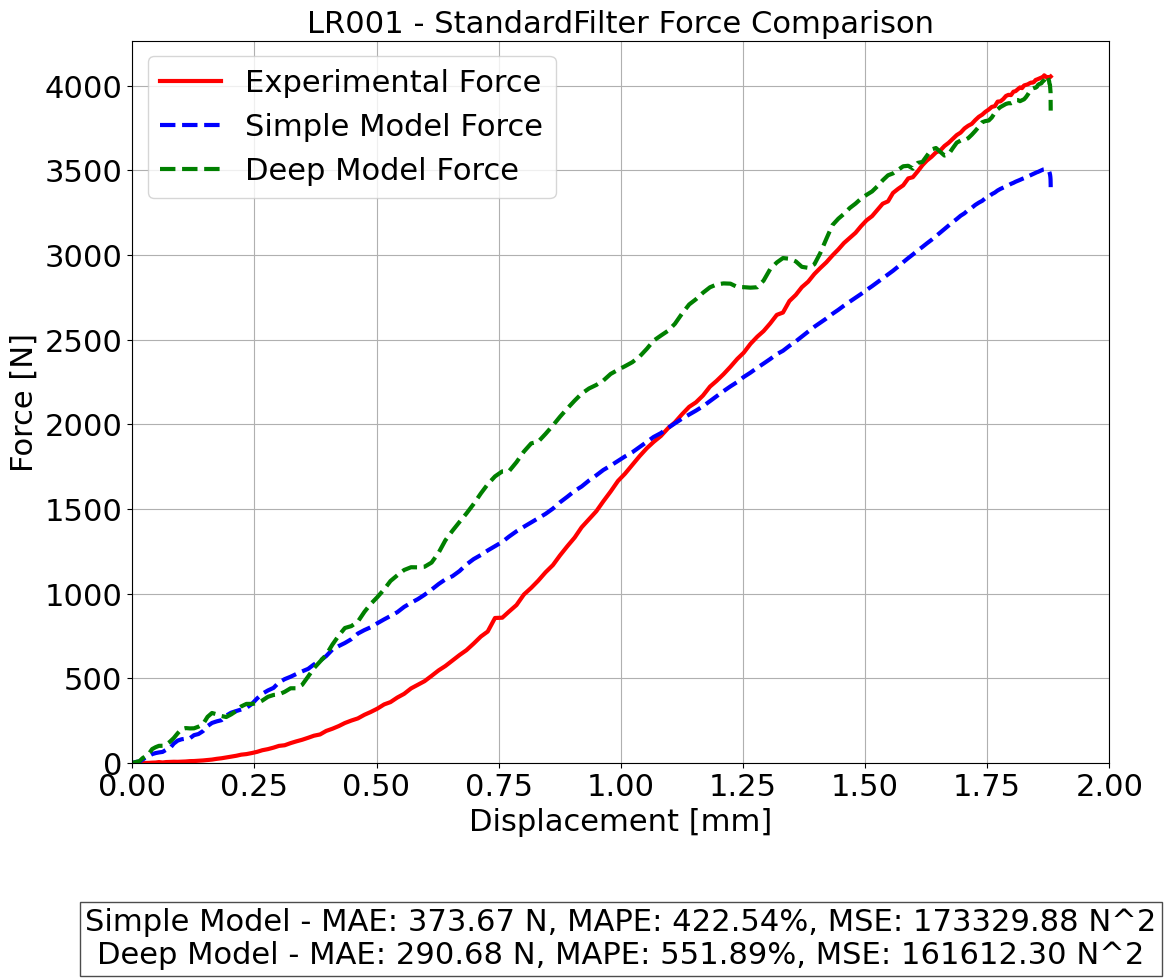
\includegraphics[width=\textwidth]{result_graphics/LR001_StandardFilter_Force_Comparison.png}
        \caption{Force Comparison}
        \label{fig:Training_No_Selector_Force}
    \end{subfigure}
    \hfill
    \begin{subfigure}[b]{0.45\textwidth}
        \centering
        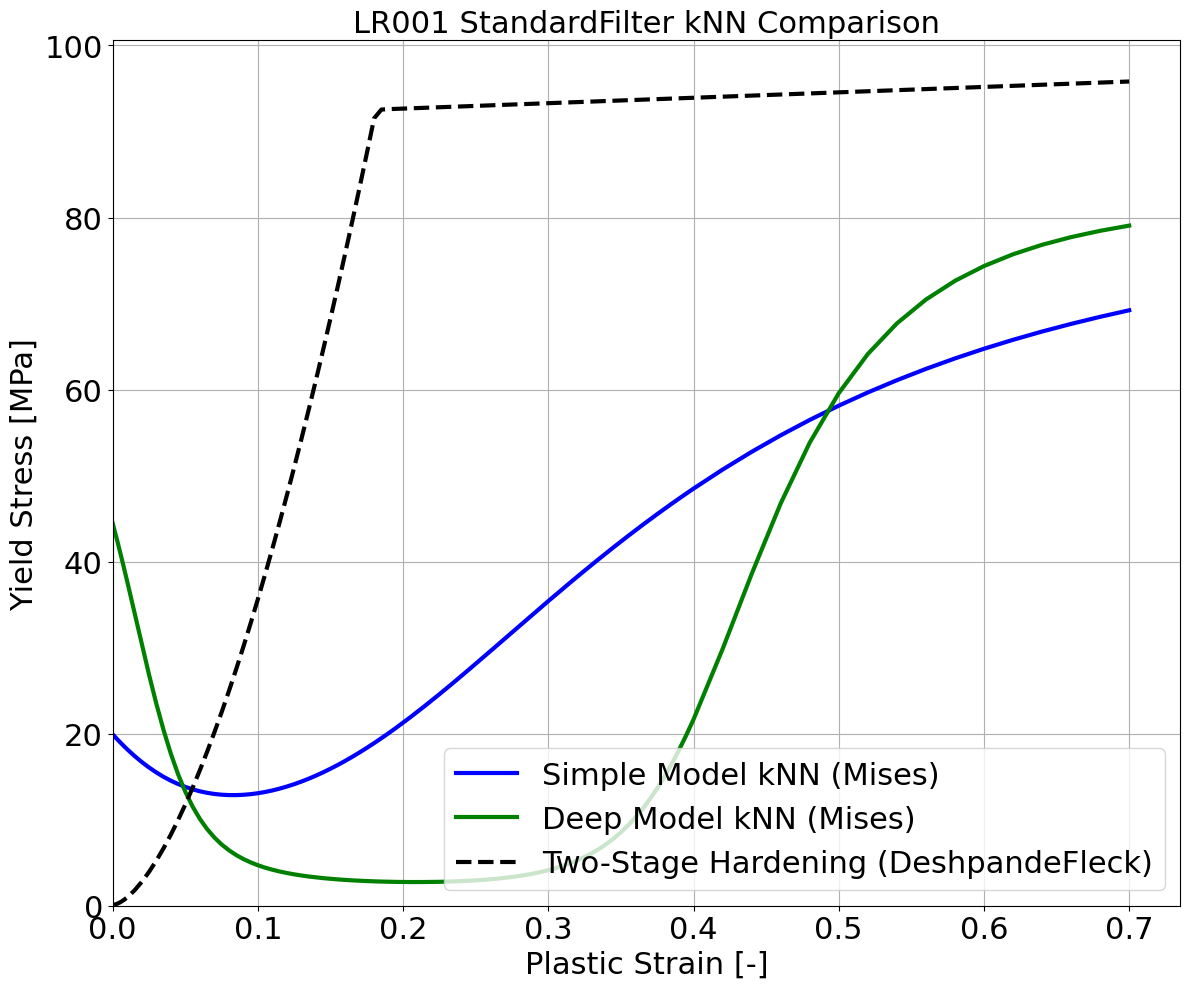
\includegraphics[width=\textwidth]{result_graphics/LR001_StandardFilter_kNN_Comparison_kNN_Comparison.png}
        \caption{kNN Comparison}
        \label{fig:Training_No_Selector_kNN}
    \end{subfigure}

    \caption{Training results without feature selector (No Selector) at LR 0.001.}
    \label{fig:Training_No_Selector}
\end{figure}

\begin{figure}[H]
    \centering
    
    % Title for the figure
    \caption*{\textbf{Training Results for Regularization}}

    % First set: Training Regularization LR 0.001
    \begin{subfigure}[b]{0.45\textwidth}
        \centering
        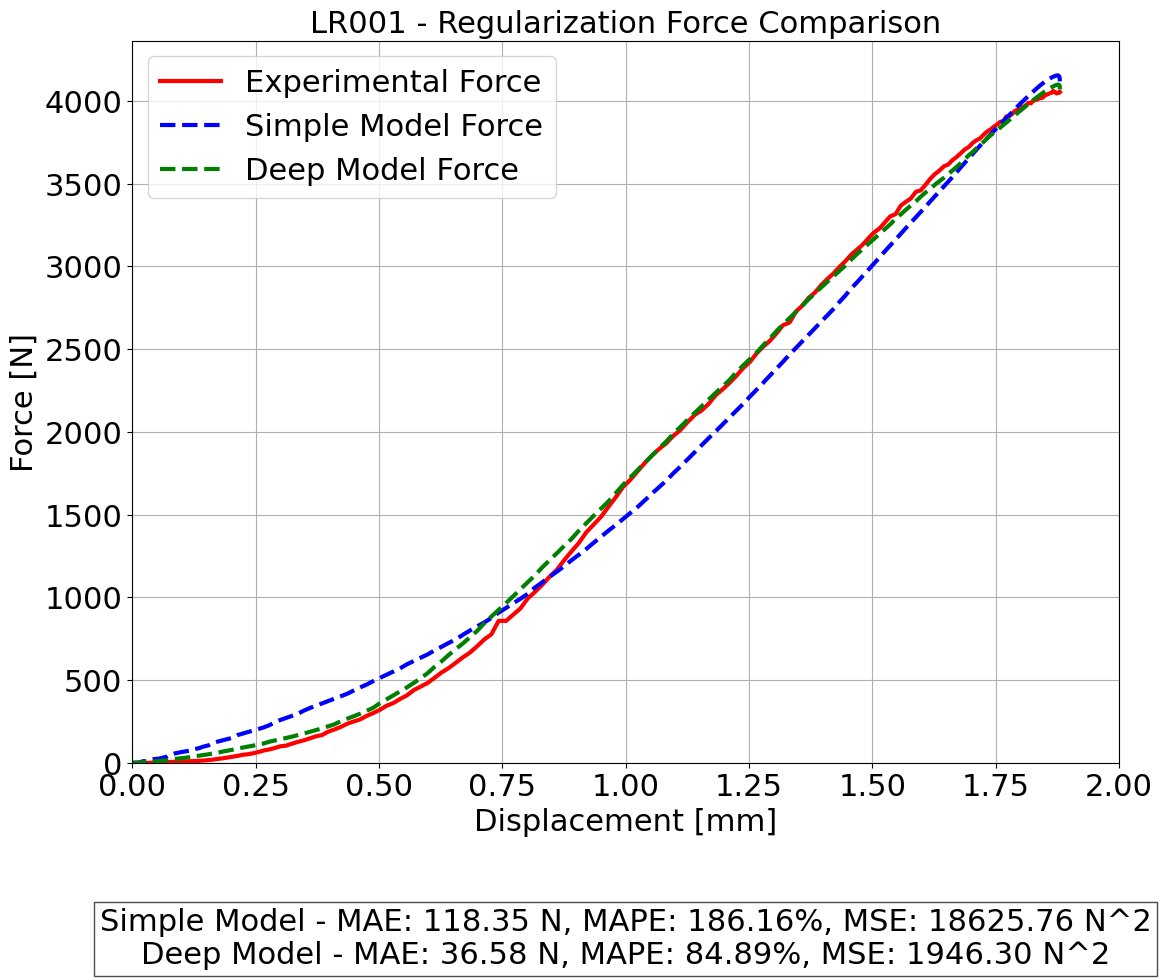
\includegraphics[width=\textwidth]{result_graphics/LR001_Regularization_Force_Comparison.png}
        \caption{Force Comparison for LR 0.001}
        \label{fig:Training_Regularization_001_Force}
    \end{subfigure}
    \hfill
    \begin{subfigure}[b]{0.45\textwidth}
        \centering
        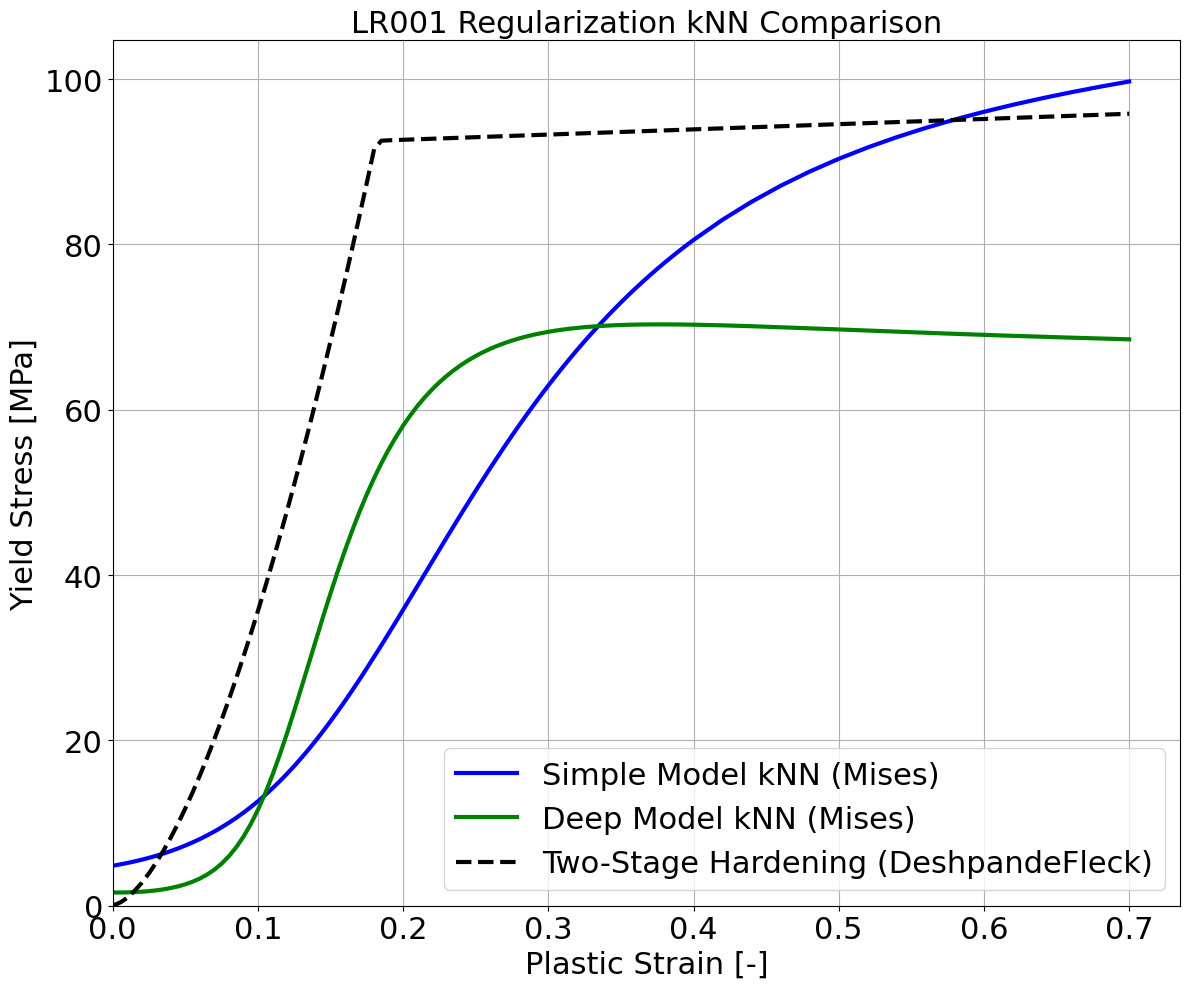
\includegraphics[width=\textwidth]{result_graphics/LR001_Regularization_kNN_Comparison_kNN_Comparison.png}
        \caption{kNN Comparison for LR 0.001}
        \label{fig:Training_Regularization_001_kNN}
    \end{subfigure}

    \vspace{1em}

    % Second set: Training Regularization LR 0.0005
    \begin{subfigure}[b]{0.45\textwidth}
        \centering
        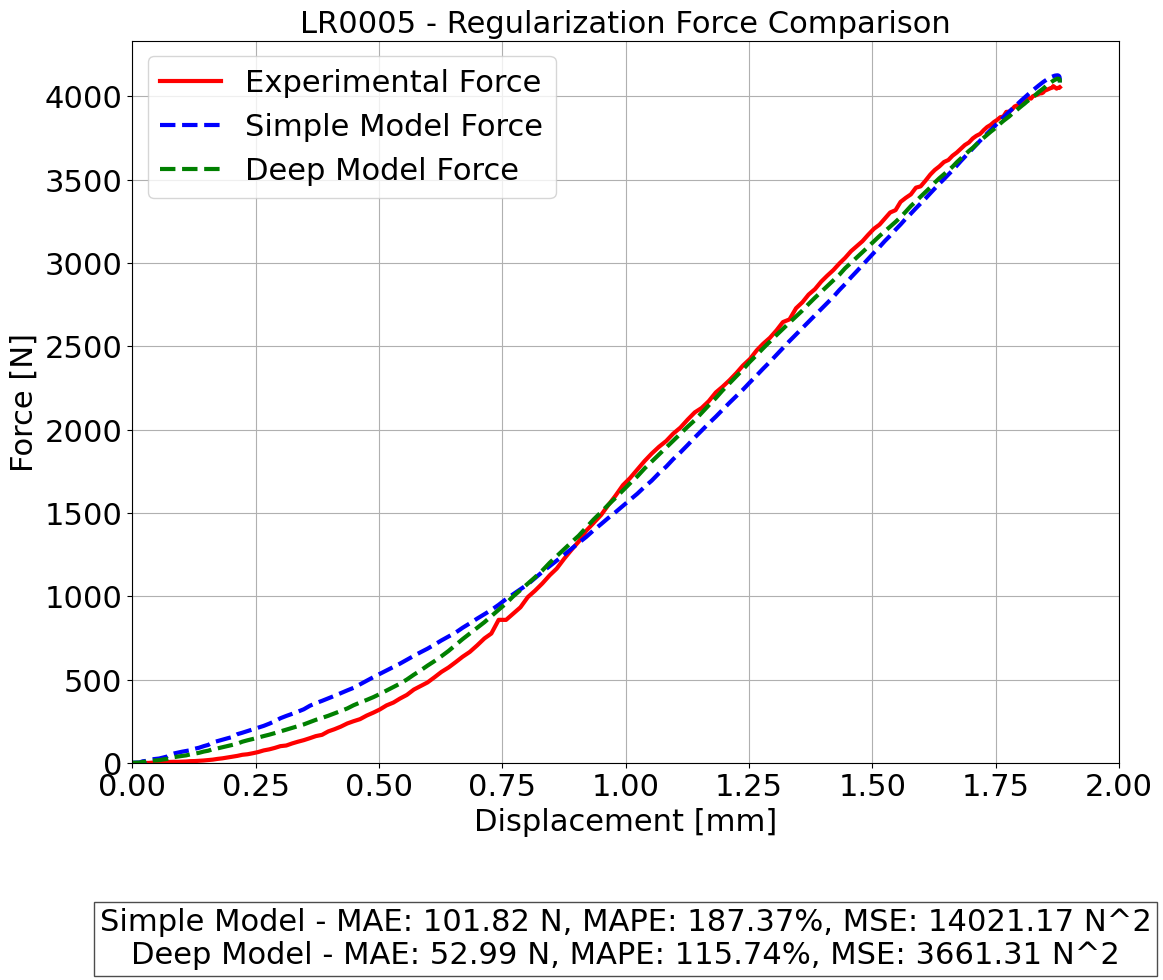
\includegraphics[width=\textwidth]{result_graphics/LR0005_Regularization_Force_Comparison.png}
        \caption{Force Comparison for LR 0.0005}
        \label{fig:Training_Regularization_0005_Force}
    \end{subfigure}
    \hfill
    \begin{subfigure}[b]{0.45\textwidth}
        \centering
        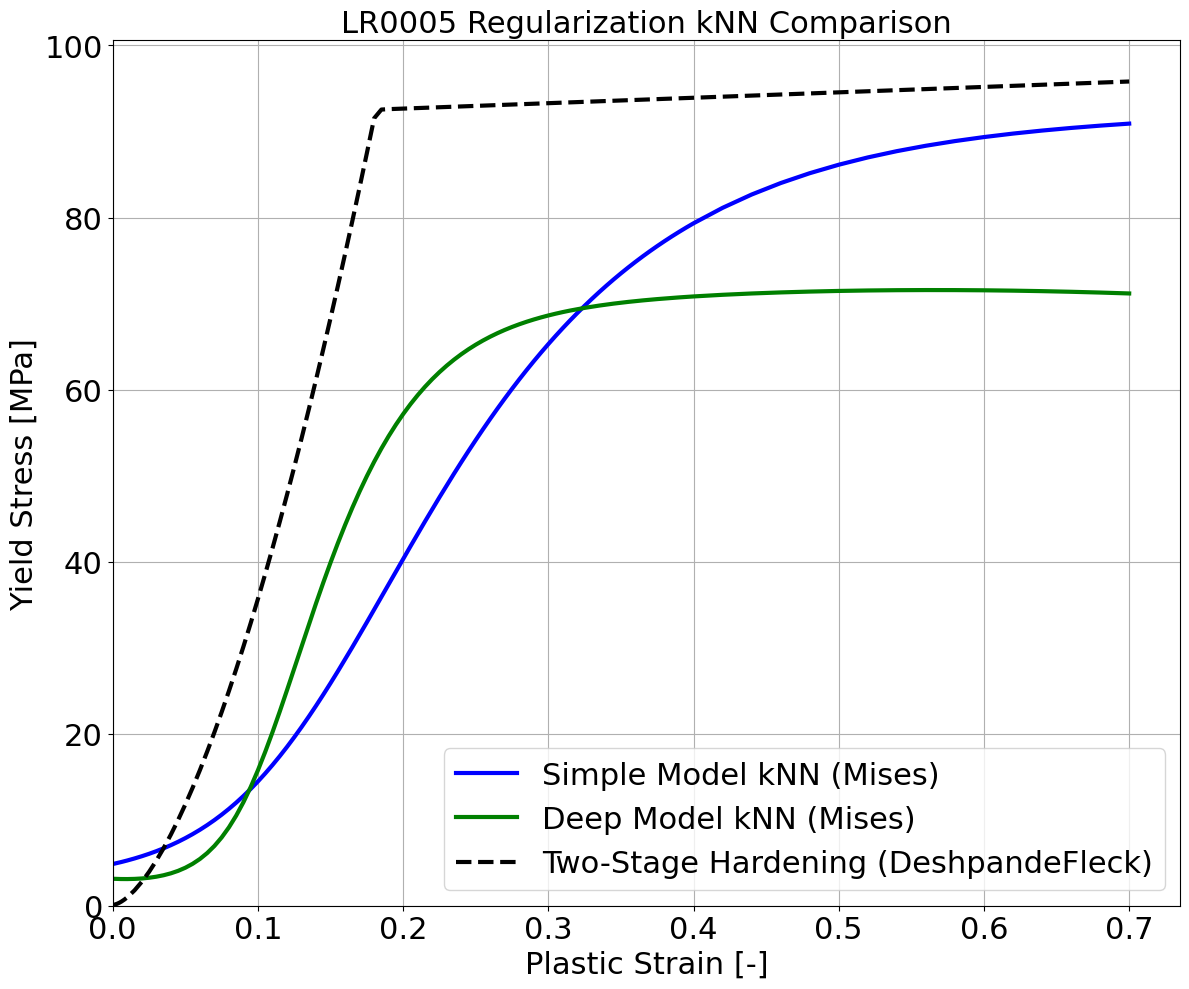
\includegraphics[width=\textwidth]{result_graphics/LR0005_Regularization_kNN_Comparison_kNN_Comparison.png}
        \caption{kNN Comparison for LR 0.0005}
        \label{fig:Training_Regularization_0005_kNN}
    \end{subfigure}

    \caption{Training results with regularization at different learning rates (LR 0.001 and LR 0.0005).}
    \label{fig:Training_Regularization}
\end{figure}

\begin{figure}[H]
    \centering
    
    % Title for the figure
    \caption*{\textbf{Training Results for Enforce Direction}}

    % First set: Training Enforce Direction LR 0.001
    \begin{subfigure}[b]{0.45\textwidth}
        \centering
        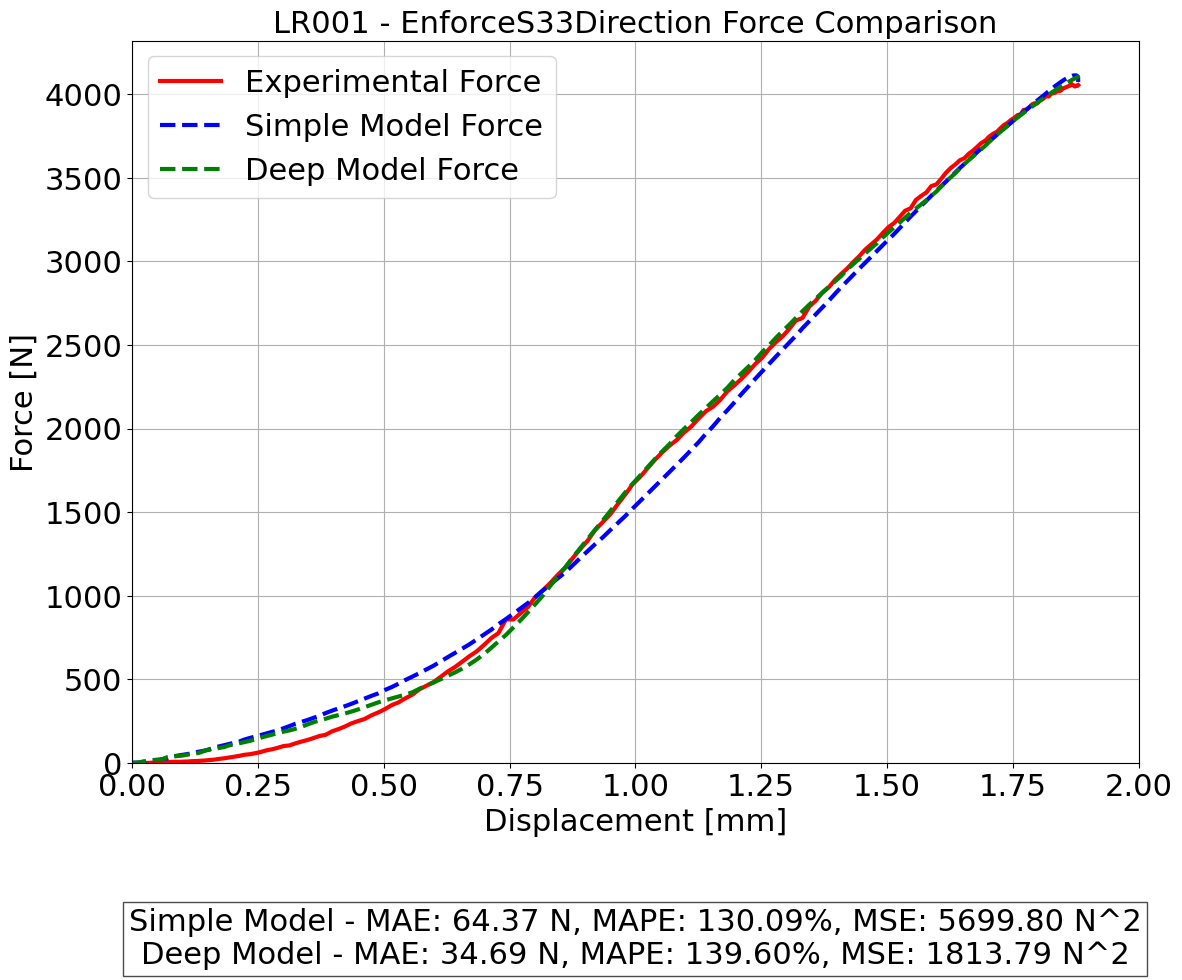
\includegraphics[width=\textwidth]{result_graphics/LR001_EnforceS33Direction_Force_Comparison.png}
        \caption{Force Comparison for LR 0.001}
        \label{fig:Training_Enforce_001_Force}
    \end{subfigure}
    \hfill
    \begin{subfigure}[b]{0.45\textwidth}
        \centering
        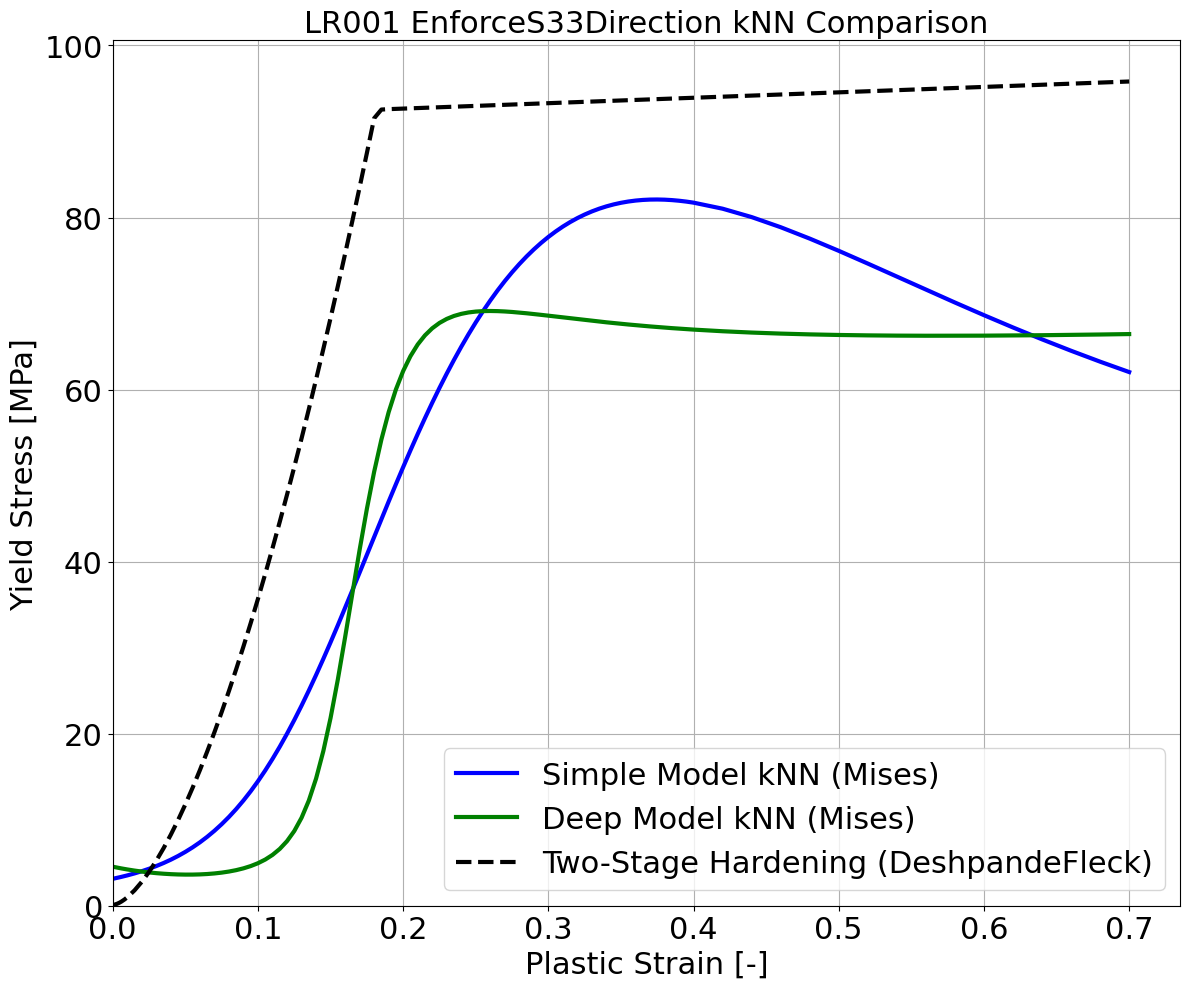
\includegraphics[width=\textwidth]{result_graphics/LR001_EnforceS33Direction_kNN_Comparison_kNN_Comparison.png}
        \caption{kNN Comparison for LR 0.001}
        \label{fig:Training_Enforce_001_kNN}
    \end{subfigure}

    \vspace{1em}

    % Second set: Training Enforce Direction LR 0.0005
    \begin{subfigure}[b]{0.45\textwidth}
        \centering
        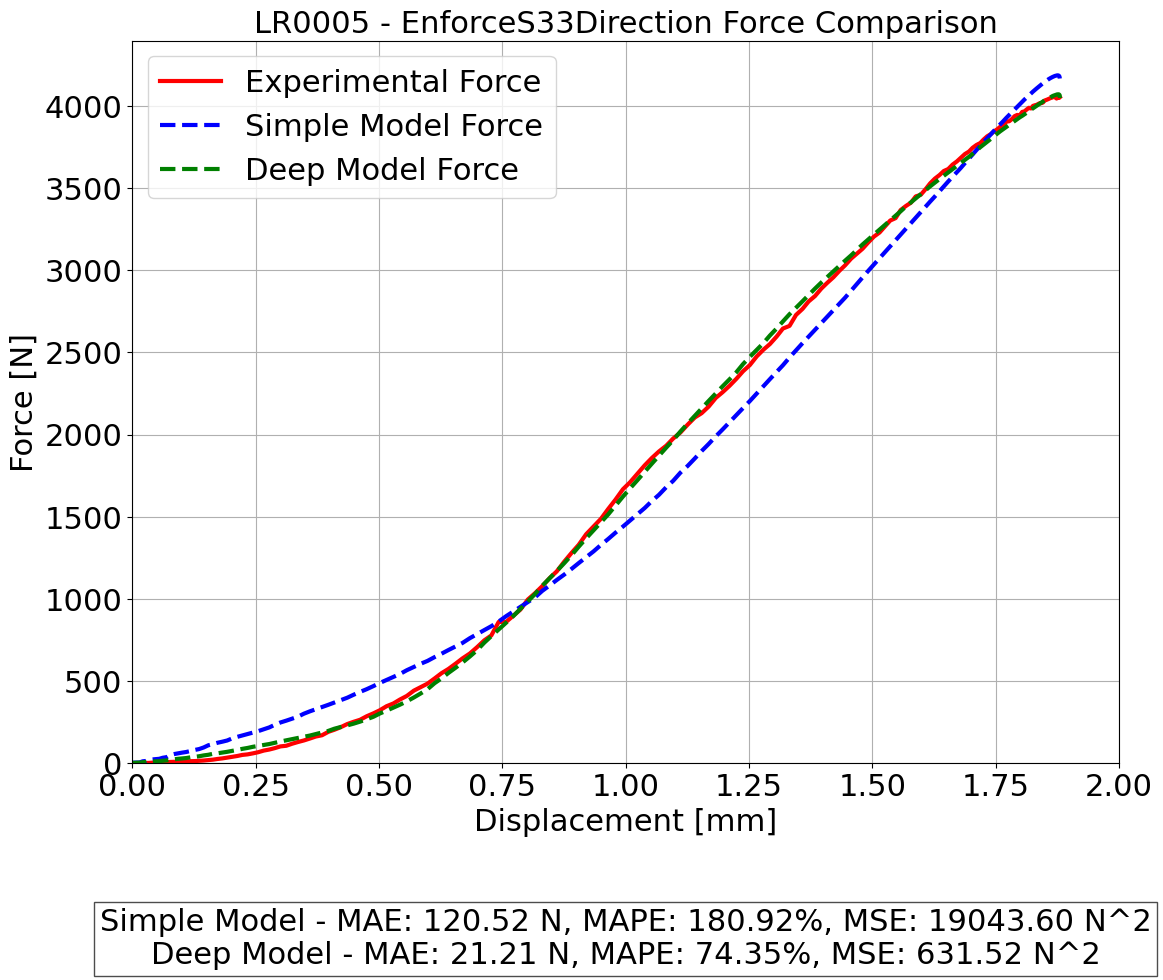
\includegraphics[width=\textwidth]{result_graphics/LR0005_EnforceS33Direction_Force_Comparison.png}
        \caption{Force Comparison for LR 0.0005}
        \label{fig:Training_Enforce_0005_Force}
    \end{subfigure}
    \hfill
    \begin{subfigure}[b]{0.45\textwidth}
        \centering
        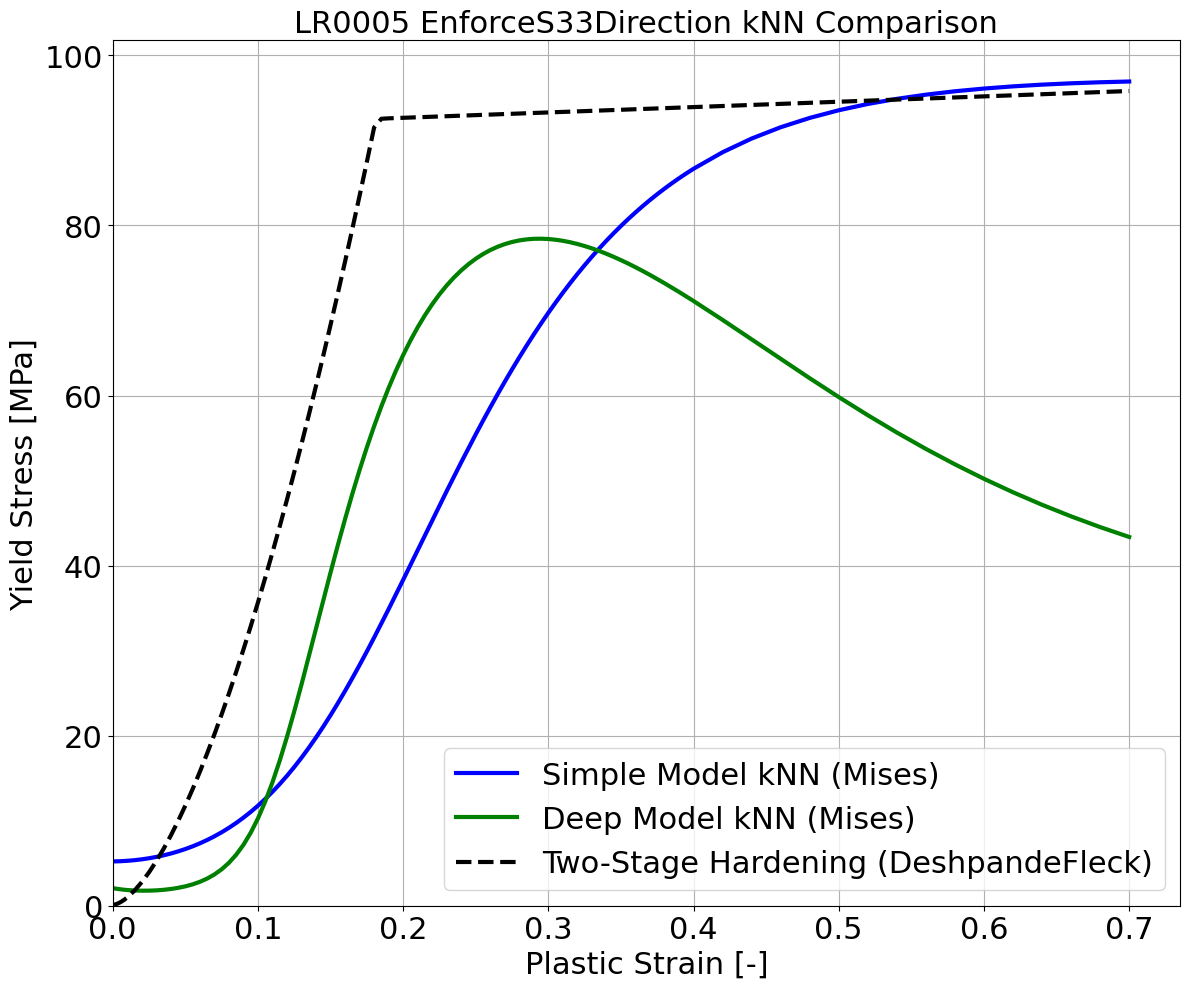
\includegraphics[width=\textwidth]{result_graphics/LR0005_EnforceS33Direction_kNN_Comparison_kNN_Comparison.png}
        \caption{kNN Comparison for LR 0.0005}
        \label{fig:Training_Enforce_0005_kNN}
    \end{subfigure}

    \caption{Training results with Enforce Direction at different learning rates (LR 0.001 and LR 0.0005).}
    \label{fig:Training_Enforce}
\end{figure}






The Key Performance Metrics and respective configurations of training runs are indicated in Table \ref{tab:performance_metrics_training}.
Figures
\ref{fig:Training_No_Selector},
\ref{fig:Training_Regularization},
\ref{fig:Training_Enforce}
show the training results for the specified method combinations. For shape comparison the two stage hardening law is included. The amplitude is not comparable as it was calibrated on a Deshpande-Fleck yield surface. Displayed are the results for the epoch, out of the total 600 epochs, that yield the lowest loss (MSE).

Further the MSE, MAPE and MAE for specified epochs and training combinations is displayed in the table.  The best run, based on the lowest performance metrics, was achieved by DeepModel with a learning rate of 0.005 and the Enforce Direction feature selector.

In contrast, the worst performance across all key performance metrics (KPM) was observed with DeepModel using a learning rate of 0.001 and the No Selector method. Overall, DeepModel with a learning rate of 0.005 and the Enforce Direction feature selector consistently produced the best results, minimizing error metrics across MSE and MAE performance measures.

The described simulations took 8 hours, running on Euler HPC, yielding a runtime of aproximately one minute per epoch.

DeepModel consistently performs better than SimpleModel, as presented in figures
\ref{fig:Training_No_Selector},
\ref{fig:Training_Regularization},
\ref{fig:Training_Enforce}
for the training runs on the H\_10 indenter except for the No Selector method. DeepModel predicted hardening laws with regularization and enforce direction are chosen to be validated on the H\_50 and C\_20 indenters. Regularization models are used as they show lower MAPE.

\subsection{Validation}


\begin{table}[H]
\centering
\begin{tabular}{|l|l|c|c|>{\columncolor[gray]{0.9}}c|>{\columncolor[gray]{0.8}}c|>{\columncolor[gray]{0.7}}c|}
\hline
\textbf{Feature Selector} & \textbf{Model} & \textbf{Learn Rate} & \textbf{Scenario} & \textbf{MSE} & \textbf{MAPE} & \textbf{MAE} \\ \hline
Enforce Direction         & DeepModel      & LR001               & C\_20             & $3.00 \times 10^7$ & 201   & 4300   \\ \cline{4-7}
                          &                &                     & H\_50             & $4.60 \times 10^5$ & 275   & 572    \\ \hline
Enforce Direction         & DeepModel      & LR0005              & C\_20             & $6.87 \times 10^6$ & 128   & 2136   \\ \cline{4-7}
                          &                &                     & H\_50             & $5.51 \times 10^4$ & 147   & 153    \\ \hline
Regularization            & DeepModel      & LR001               & C\_20             & $1.92 \times 10^7$ & 122   & 3281   \\ \cline{4-7}
                          &                &                     & H\_50             & $2.02 \times 10^6$ & 138   & 1049   \\ \hline
Regularization            & DeepModel      & LR0005              & C\_20             & $2.43 \times 10^7$ & 168   & 3562   \\ \cline{4-7}
                          &                &                     & H\_50             & $6.79 \times 10^5$ & 229   & 663    \\ \hline
\end{tabular}
\caption{Performance metrics for DeepModel validation (rounded to 3 digits)}
\label{tab:performance_metrics_valid}
\end{table}

Key performance metrics of validation experiments are presented in Table \ref{tab:performance_metrics_valid}. The lowest MSE for the cylindrical and hemispherical indentation is achieved by the best training configuration (Enforce Direction, DeepModel, LR0005). As for the training runs the MAPE is lower for Regularization than for Enforce Direction.
Figure \ref{fig:Validation_Comparison}
shows validation results for both learn rates across configurations in one chart.

\begin{figure}[H]
    \centering
    \caption*{\textbf{Validation Results}}
    % First set: Validation Regularization
    \begin{subfigure}[b]{\textwidth}
        \centering
        \begin{minipage}{0.49\textwidth}
            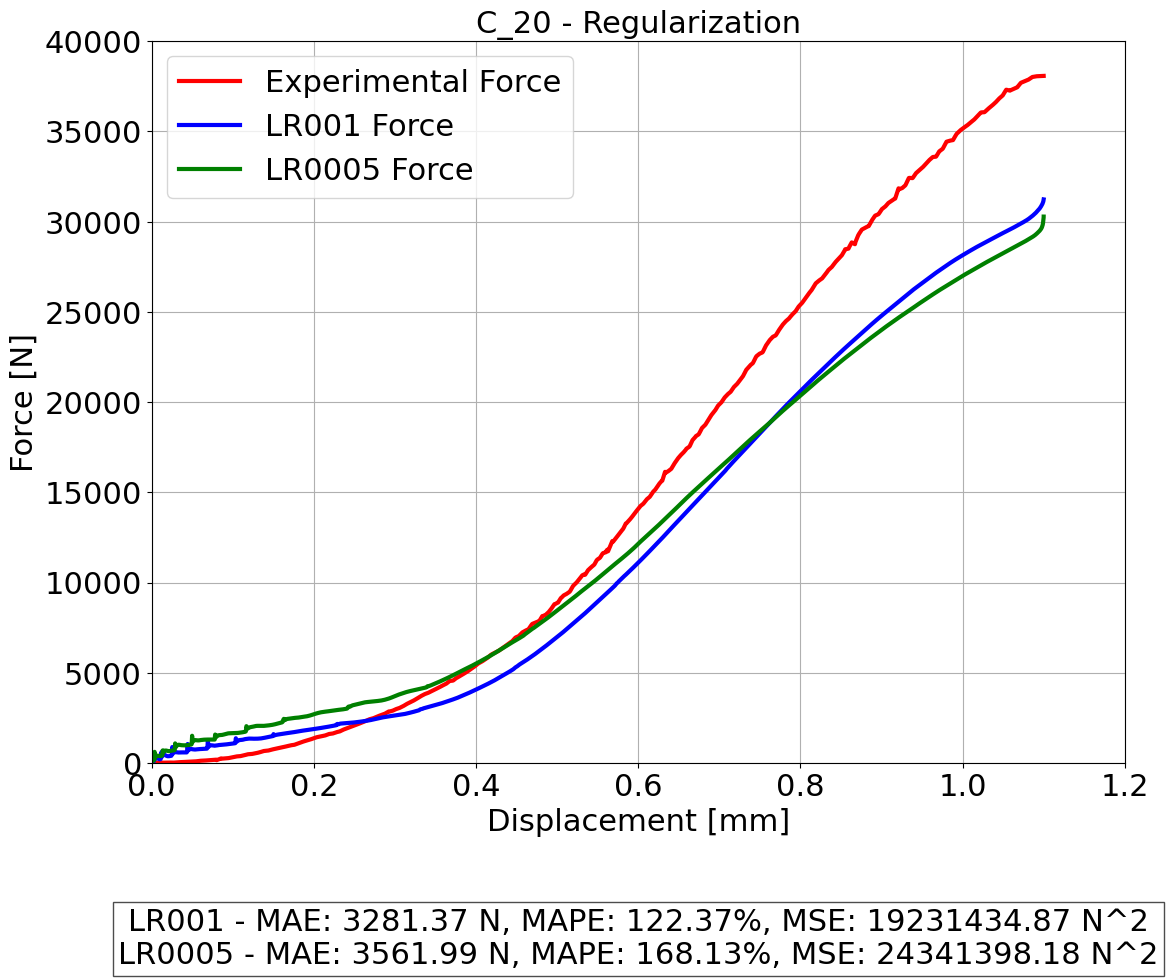
\includegraphics[width=\textwidth]{result_graphics/C_20_RegularizationForce_Comparison.png}
        \end{minipage}
        \hfill
        \begin{minipage}{0.49\textwidth}
            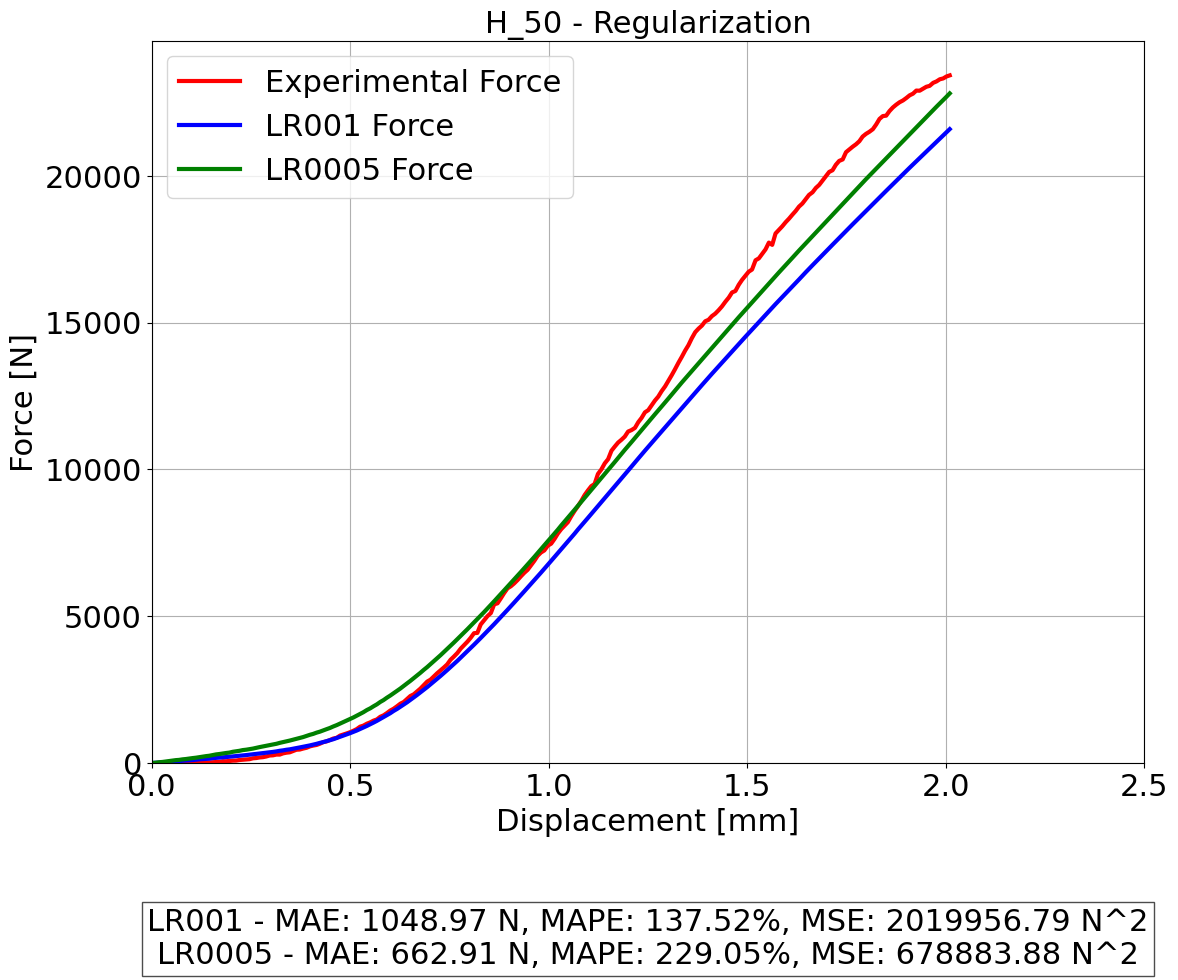
\includegraphics[width=\textwidth]{result_graphics/H_50_RegularizationForce_Comparison.png}
        \end{minipage}
        \caption{Regularization}
        \label{fig:SimpleModel_Training_Regularization_LR0005}
    \end{subfigure}
    
    \vspace{1em} % Adds space between the subfigures
    
    % Second set: Validation Enforce Direction
    \begin{subfigure}[b]{\textwidth}
        \centering
        \begin{minipage}{0.49\textwidth}
            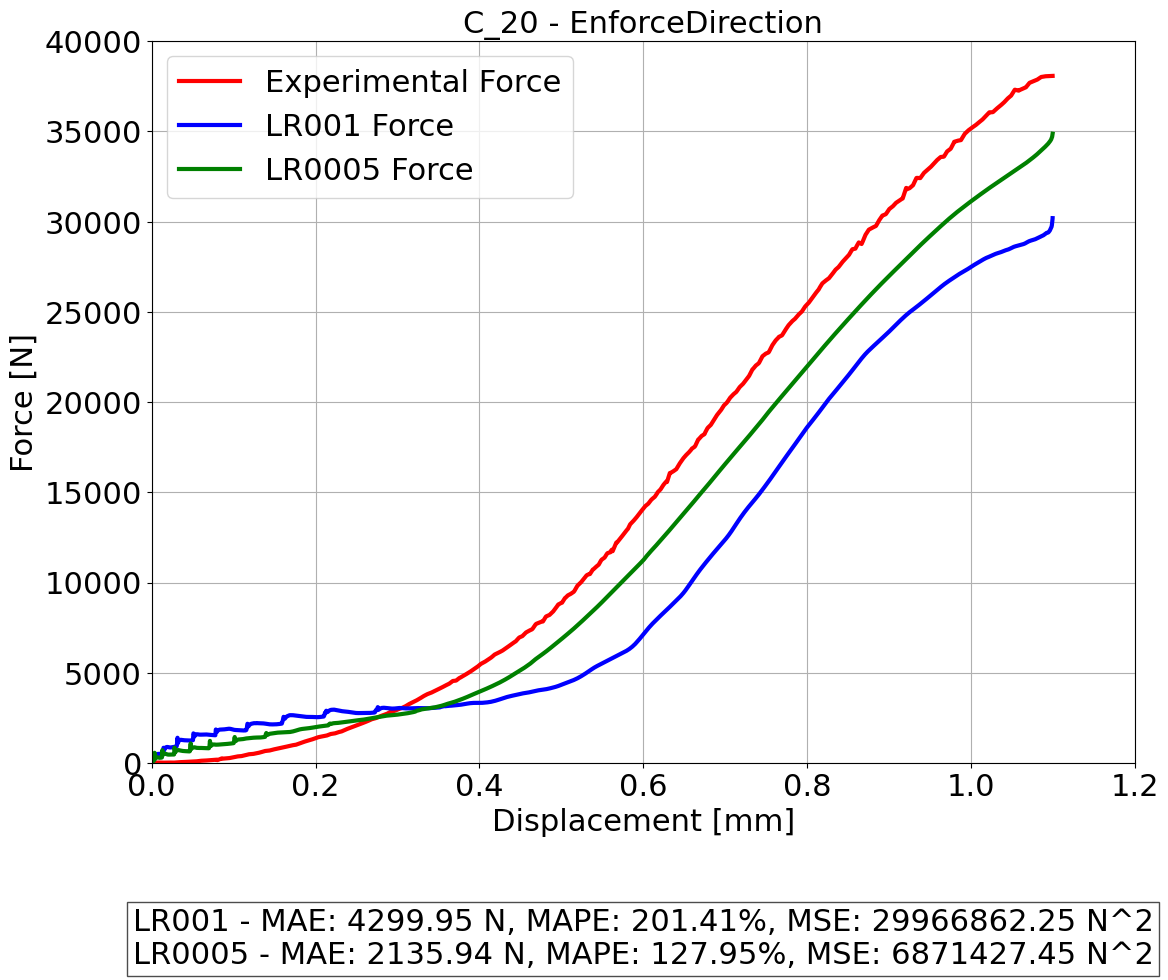
\includegraphics[width=\textwidth]{result_graphics/C_20_EnforceDirectionForce_Comparison.png}
        \end{minipage}
        \hfill
        \begin{minipage}{0.49\textwidth}
            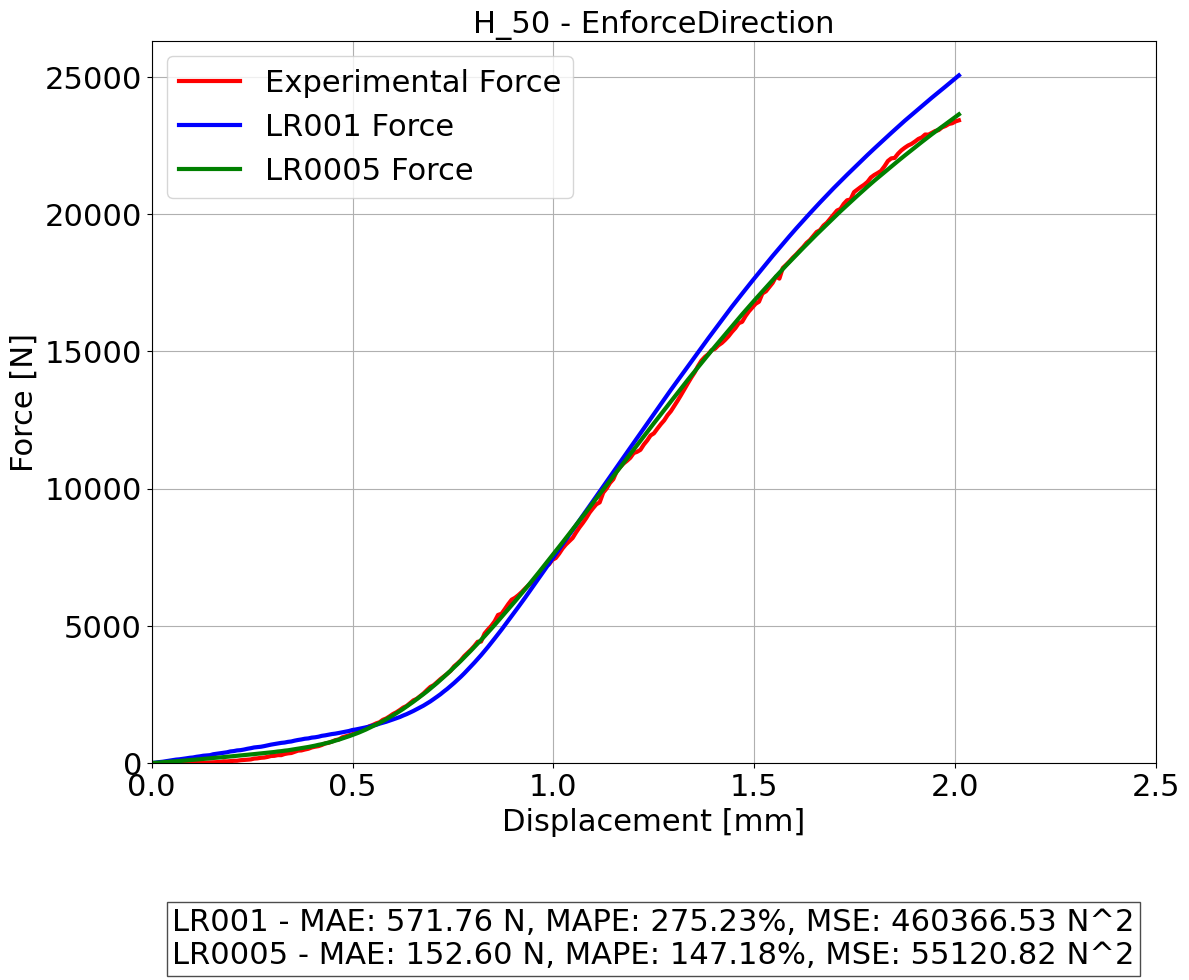
\includegraphics[width=\textwidth]{result_graphics/H_50_EnforceDirectionForce_Comparison.png}
        \end{minipage}
        \caption{Enforce Direction}
        \label{fig:SimpleModel_Training_Regularization_LR001}
    \end{subfigure}
    \caption{Validation results for selected hardening laws}
    \label{fig:Validation_Comparison}
\end{figure}

\section{Discussion}
% Discussion
The calibration process using \textit{DeepModel} is feasible but highlights limitations when using configurations such as no selector, which yields no successful neural network calibration, particularly for deeper models. This is likely due to overfitting caused by unsmooth data or coarse meshing. The gradient 
$\frac{\partial \sigma_{33}}{\partial \sigma_{\text{vM}}}$
is also likely impacted by the unsmooth data, leading to poor results.

In contrast, the enforce direction feature selector produces better results, achieving more accurate gradient representations when simplifying boundary conditions, such as uniaxial compression. However, it occasionally results in decreasing yield stress at higher strains. regularization shows merit in handling these issues, especially at lower displacements, where it provides a more stable force match.

A key issue is the uneven force response at lower displacements, resulting in a high MAPE across the force-displacement curve. This is likely caused by the inclusion of more contact elements at higher displacements, leading to an uneven gradient distribution. If a smoother and evenly distributed gradient representation for the loss function could be achieved, convergence issues would likely be reduced, leading to stable and reliable training.

The oscillating loss curves are concerning, likely due to large steps in the gradient descent or uneven feature distribution. A method to improve feature selection and machine learning hyperparameters could stabilize the optimization process, leading to a more accurate force response.

\section{Conclusion}
% Conclusion
The main objective of this thesis was to investigate the use of deep learning models, specifically fully connected neural networks (FCNN), to predict the hardening law of lithium-ion batteries. The goal was to optimize force matching in simulations by predicting yield stress from plastic strain.

This research demonstrated that:
\begin{itemize}
    \item The calibration process using DeepModel was feasible, achieving successful force and displacement matching.
    \item Enforce direction outperformed other configurations, particularly in terms of accuracy in validation runs such as {C\_20} and {H\_50}, while  regularization showed better performance at lower displacements.
    \item Challenges with convergence and oscillating loss curves were encountered, particularly in the no selector configuration.
\end{itemize}

This study contributes to the field of material science and battery technology by applying deep learning techniques to model complex material behavior. The successful application of FCNN models to simulate the hardening behavior of pouch cells presents a new approach to improving computational efficiency in simulation environments like \textit{Abaqus}. Furthermore, the framework developed in this work may be applied to any calibration process if an adequate loss function gradient is identified. Using more advanced yield surfaces beyond the \textit{von Mises criterion} could further enhance efficiency and reduce the need for manual calibration.

Several limitations are identified, including unstable training behavior, lower accuracy at reduced displacements, and issues arising from mesh size and data density constraints. Additionally, the \textit{von Mises yield criterion} may limit the model’s ability to capture certain material behaviors, and future work should explore more advanced models like \textit{Deshpande-Fleck’s crushable foam} for improved results.

In conclusion, this thesis lays a foundation for further exploration of deep learning models in material simulation. While challenges remain in achieving smooth and reliable training outcomes, the work opens new possibilities for improving the accuracy of battery simulations and extending the approach to other material systems.

\newpage
\section{Outlook}
This section outlines six key strategies deemed most relevant and efficient for advancing the research. These methods focus on enhancing the model’s generalization, accuracy, and overall performance through the incorporation of experimental diversity, alternative loss function approaches, and optimized training strategies. By addressing current limitations and introducing more advanced techniques, these strategies aim to improve the model's predictive power and robustness for future applications.

\begin{enumerate}

    \item \textbf{Incorporate Multiple Experiments for Training}
    \begin{itemize}
        \item \textbf{Issue}: Using a single test size limits the model's ability to generalize across different scenarios. The physical relationships the model learns may be biased towards specific configurations, reducing its accuracy when applied to varying setups.
        \item \textbf{Aim}: Incorporate data from multiple experiments with different test sizes and configurations. By training the model on diverse experiments, it can better capture the general relationships between strain, stress, and force, improving its ability to generalize to unseen cases.
        \item \textbf{Expected Outcome}: The model will become more robust and versatile, capable of making accurate predictions across different test setups and sizes. This approach will reduce overfitting to a single test size and improve the model's overall performance, especially in scenarios with varying strain or displacement conditions.
    \end{itemize}
    
    \item \textbf{Investigate Alternative Loss Functions}
    \begin{itemize}
        \item \textbf{Issue}: The current loss function, such as Mean Squared Error (MSE), may not provide optimal force matching at lower displacements.
        \item \textbf{Aim}: Explore alternative loss functions, such as weighted loss functions or those that consider the Mean Absolute Percentage Error (MAPE), to improve force matching at lower displacements.
        \item \textbf{Expected Outcome}: A more accurate force match across all displacements. Since force error at lower displacements is expected to propagate into higher displacements, weighted loss functions might help mitigate this by focusing on minimizing errors early on. As the number of elements grows with indenter displacement due to the geometry of the test, having more accurate strain predictions in early stages can prevent accumulation of errors at larger displacements.
    \end{itemize}
    

    \item \textbf{Explore Framework Configuration for Monotonically Converging Training Behavior}
    \begin{itemize}
        \item \textbf{Issue}: Training configurations often oscillate or diverge after finding a local minimum, instead of adjusting slightly to further optimize it. This can be observed in the training behavior over all epochs, where the model tends to converge to a solution that provides an adequate force match at higher displacements. However, issues arise when the gradients from lower displacements start to influence the model more significantly.
        
        \item \textbf{Aim}: Identify a framework configuration that ensures monotonically converging training behavior by addressing the imbalance between gradients at lower and higher displacements. The goal is to manage how the gradient for input features (strains) at lower displacements affects model updates without disproportionately impacting the force error.
        
        \item \textbf{Expected Outcome}: Achieve stable and consistent training progress, reducing the risk of oscillation or divergence. By addressing the local minima issue and controlling how predicted yield stresses for lower strains are adjusted, the model can prevent disproportionate force errors. This is crucial since yield stress at lower strains has a more significant effect on force predictions when fewer elements are involved (lower displacements) and can cause cascading issues as the number of elements grows at higher displacements.
    \end{itemize}
    
\newpage
    \item \textbf{Investigate Increasing Element Number / Finer Mesh}
    \begin{itemize}
        \item \textbf{Issue}: The current element number and mesh size may not provide optimal resolution for the framework's performance.
        \item \textbf{Aim}: Increase the element number for smoother optimization results. Sample gradients when the element count exceeds a threshold to ensure an even gradient distribution across displacements.
        \item \textbf{Expected Outcome}: Achieve smoother edges, filters, and gradient distributions across plastic strains and displacements. Gradient sampling will help mitigate spikes and uneven distributions, though this approach may increase computational cost and slow down simulations.
    \end{itemize}

    \item \textbf{Explore Combination of Selection Methods: Regularization and Enforce Direction}
    \begin{itemize}
        \item \textbf{Issue}: The regularization selector adds features for 0 strain to ensure a constant number of features per displacement. While this approach leads to fast gradient convergence, it results in reduced accuracy compared to the enforce direction selector, which converges more slowly but provides better accuracy.
        \item \textbf{Aim}: Combine the regularization selector, which maintains constant features per displacement, with the enforce direction method to balance fast convergence and accurate force predictions.
        \item \textbf{Expected Outcome}: Achieve a balance between convergence speed and prediction accuracy. By using both methods, the model should converge faster than using enforce direction alone, while maintaining better accuracy than regularization alone. This ensures a stable number of features per displacement while improving overall performance.
    \end{itemize}

    \item \textbf{Learn Loss Gradient Using a Second Model Instead of an Analytical Solution}
    \begin{itemize}
        \item \textbf{Issue}: The gradient of the loss with respect to yield stress is typically dependent on the yield surface, making the analytical gradient description limited by the specific yield surface used. Further the analytical solution only gives an aproximation of the gradient which might be more complex.
        
        \item \textbf{Aim}: Use a machine learning (ML) model to describe the gradient, making the loss function independent of the yield surface. The model could learn the relationship between yield stress predictions and resulting force errors by running multiple simulations. All important metrics, such as the complete stress tensor and different equivalent stresses (\textit{vergleichsspannungen}), could be used as inputs to capture more complex relationships.
        \item \textbf{Expected Outcome}: By using a machine learning-based approach, the model could find complex relationships between input features and the resulting gradients that are not captured by the filter mechanism or the analytical gradient description. This double ML approach (using ML for both predictions and gradient calculations) would enable the model to handle more complex optimization scenarios and potentially improve overall accuracy.
    \end{itemize}
\end{enumerate}
\newpage
\section*{Acknowledgements}
First and foremost, I would like to express my sincere gratitude to Prof. Dr. Dirk Mohr for granting me the opportunity to conduct my research in his lab. His support has been invaluable in allowing my pursuit of this work.

I would also like to thank my advisors, Thomas Tancogne-Dejean and Xueyang Li, for their insightful discussions, guidance, and encouragement throughout the research process. Their expertise and mentorship have been essential to the development of this thesis.

A special thanks to my co-advisor, Emmanouil Sakaridis, for his technical support and numerous inputs, which greatly contributed to the progress of this work.

I am grateful to the entire team at the \textit{Artificial Intelligence in Mechanics and Manufacturing} lab for providing a collaborative environment that enabled me to carry out this research effectively.

I thoroughly enjoyed my research journey and am particularly grateful for the powerful technology of large language models (LLMs) and AI tools such as DALL-E. These cutting-edge tools enabled me to iterate quickly through my research and rapidly acquire advanced Python skills and machine learning knowledge.

Last but not least, I would like to thank my friends, Malin Karlsson and Max Haberthür, for their invaluable help in proofreading and offering editing suggestions.
\newpage
\bibliography{research_sources}

\end{document}
